\documentclass[12pt, a4paper]{article}

\usepackage[utf8]{inputenc}
\usepackage[T1]{fontenc}
\usepackage{times} % Times New Roman equivalent
\usepackage{geometry}
\usepackage{graphicx}
\usepackage{amsmath}
\usepackage{booktabs}
\usepackage{caption}
\usepackage{float}
\usepackage[hidelinks]{hyperref}
\usepackage{fancyhdr}
\usepackage{cleveref}
\usepackage{parskip}
\usepackage{tabularx}
\usepackage{siunitx}
\usepackage{xurl}
\usepackage{comment}
\usepackage{multicol}

\geometry{margin=1in}
\urlstyle{same}
\numberwithin{table}{section}
\numberwithin{figure}{section}
\renewcommand{\refname}{}
\captionsetup[figure]{justification=centering,
hypcap=false}

\pagestyle{fancy}
\fancyhf{}
\fancyfoot[C]{\thepage}
\renewcommand{\headrulewidth}{0pt}

\begin{document}

\begin{titlepage}
    \centering
    \vspace*{\fill}

\begin{figure}[H]
    \centering
    
\includegraphics[width=0.5\linewidth]{logo.png}
\end{figure}
    
    {\large Department of Electrical and Electronics Engineering} \\
    \vspace{2cm}
    {\Large \textbf{ELE 214: Electronics Laboratory - I}} \\
    \vspace{0.5cm}
    {\Large \textbf{Multistage Amplifier Design and Fabrication}} \\
    \vspace{1cm}
    {\large Term Project - Spring 2026} \\
    \vspace{6cm}
    \textbf{Student:} Baturay Kafkas \\
    \textbf{Student ID:} 2240357068\\
    \vspace*{\fill}
    %\textbf{Date:} \today
\end{titlepage}

\newpage
\setcounter{page}{2}

\tableofcontents
\newpage

\section{Abstract}

This project demonstrates the knowledge gathered in ELE230 - Electronics I, ELE214 - Electronics Laboratory I, and ELE226 - Circuit Theory II in the 2025-2026 spring academic term. It allows the student to gain hands-on experience with electrical components, acquire skills, and put theory into practice. The lists of figures and tables are given in \autoref{subsec:appendix_b}.

\section{Objective}

The goal of this project is to be able to use the two types of transistors, BJT and MOSFET, and other electrical components to form up an audio amplifier with a specific gain. In this project, the use of operational amplifier is to be avoided. The system must include a buffer stage, an adjustable band-pass equalizer, and a gain stage.

As instructed, at least one BJT and one MOSFET should be used. In this project, the BJT is going to be used for buffer stage and MOSFET for the gain stage.

\subsection{Buffer Stage}

Since this stage has unity gain, an emitter follower configuration may be used. It has a large input resistance and low output resistance~\cite{1}.

\subsection{Equalizer Stage}

This stage is to be designed using two capacitors. An RLC circuit could also do the same job. Since a capacitor can be easily found on the market, it is preferred to utilize capacitors instead.

\subsection{Gain Stage}

Our aim is to increase the output voltage. Therefore, a common-source configuration can be used. In this stage, the audio is ensured to be amplified. Since no speaker is going to be used, we can directly measure the output voltage in this stage.

\section{Research and Analytical Calculations}

\subsection{Definitions}

\begin{itemize}
    \item \textbf{Amplifier:} An electronic device that is used to increase the magnitude of an input signal.
    \item \textbf{Buffer stage:} The stage that transfers a signal from one stage to another without altering its voltage level (i.e., it has unity gain) while preventing interaction between the stages.
    \item \textbf{Equalizer stage:} A circuit or processor that attenuates or boosts specific frequencies. It determines the frequency range that will be conveyed to the other stage.
    \item \textbf{Gain stage:} The stage where the signal level is increased to a desired value.
    \item \textbf{Multistage amplifier:} An amplifier formed by connecting two or more amplifier stages in series. The stages are said to be in a cascade connection.
    \item \textbf{Role of Capacitors:} In an audio amplifier, capacitors are used mainly in two roles: coupling capacitors and bypassing capacitors.

    Coupling capacitors pass AC signals while blocking DC between stages and prevent bias disturbance.
    
    Bypass capacitors stabilize gain by providing a low-impedance path to ground for AC, disabling the degeneration resistor.
    \item \textbf{MOSFET vs BJT Differences:} \autoref{tab:bjt_mosfet} and ~\autoref{fig:bjt_mosfet} show the differences.
\end{itemize}

\begin{table}[h]
\caption{Comparison between BJT and MOSFET}
\centering
\renewcommand{\arraystretch}{1.3}
\begin{tabular}{|c|p{4.5cm}|p{5.7cm}|}
\hline
\textbf{Feature} & \textbf{BJT} & \textbf{MOSFET} \\
\hline
Classification & NPN, PNP & NMOS, PMOS \\
\hline
Control Type & Current-controlled device & Voltage-controlled device \\
\hline
Terminals & Emitter, base, collector & Source, gate, drain, body \\
\hline
Input Impedance & Low (k$\Omega$ range) & Very high (M$\Omega$ to G$\Omega$) \\
\hline
Input Current & Continuous base current & Almost zero gate current \\
\hline
Regions & Active, saturation, cutoff & Linear (ohmic, triode), saturation \\
\hline
Power Consumption & Higher & Lower \\
\hline
Thermal Stability & Poor & Better \\
\hline
Noise Performance & Higher noise & Lower noise \\
\hline
Typical Applications & Analog amplifiers & Digital circuits, power electronics \\
\hline
\end{tabular}
\label{tab:bjt_mosfet}
\end{table}

\begin{figure}[H]
    \centering
    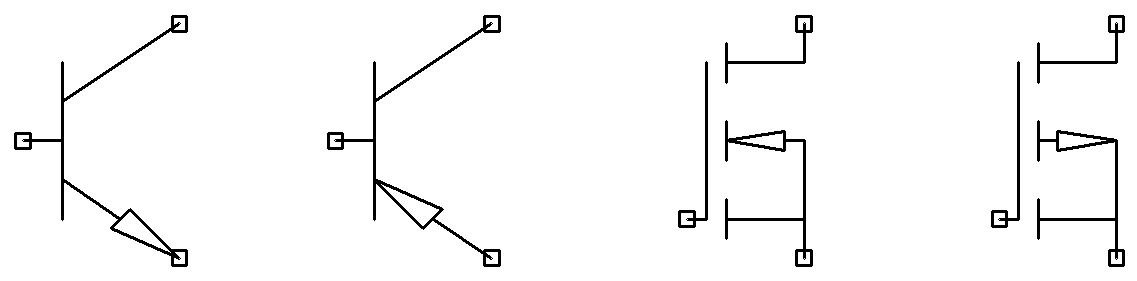
\includegraphics[width=0.8\textwidth]{bjt_mosfet.png}
    \caption{LTspice Symbols From Left to Right: NPN, PNP, NMOS, PMOS}
    \label{fig:bjt_mosfet}
\end{figure}

\subsection{Transistor Choice}

In this design, we decided to use the 2N2222 and 2N7000 models. They are widely available, low-cost, and well-documented components that are suitable for an electronics project that a student may design. The BJT provides a reliable solution for small-signal amplification. As for the MOSFET, it offers efficient switching with minimal drive requirements and enhances the output voltage.

\autoref{tab:2N2222}~\cite{2}, \autoref{fig:fig2}, and \autoref{fig:fig3} show the properties of the 2N2222/2N2222A transistor. ~\autoref{tab:2N7000}~\cite{3} shows the properties of the 2N7000 transistor.

\newpage

\vspace{\fill}
\begin{comment}
\begin{table}[h!]
    \caption{Electrical Characteristics of 2N2222A ($T_A = 25^\circ C$ unless otherwise noted)}
    \label{tab:2N2222A}
    \small
    {\centering
    \begin{tabularx}{\textwidth}{X c c c c}
        \toprule
        \textbf{Characteristic} & \textbf{Symbol} & \textbf{Min} & \textbf{Max} & \textbf{Unit} \\ 
        \midrule
        \multicolumn{5}{l}{\textbf{OFF CHARACTERISTICS}} \\
        Collector--Emitter Breakdown Voltage \\\quad ($I_C = 10$ mAdc) & $V_{(BR)CEO}$ & 50 & -- & Vdc \\
        Collector--Base Cutoff Current& $I_{CBO}$ &  &  &  \\
        \quad($V_{CB} = 75$ Vdc) & & -- & 10 & $\mu$Adc \\
        \quad($V_{CB} = 60$ Vdc) & & -- & 10 & nAdc \\
        Emitter--Base Cutoff Current & $I_{EBO}$ & & & \\
        \quad($V_{EB} = 6.0$ Vdc) & & -- & 10 & $\mu$Adc \\
        \quad($V_{EB} = 4.0$ Vdc) & & -- & 10 & nAdc \\
        Collector--Base Cutoff Current \\\quad ($V_{CE} = 50$ Vdc) & $I_{CES}$ & -- & 50 & nAdc \\
        \midrule
        \multicolumn{5}{l}{\textbf{ON CHARACTERISTICS} (Note 1)} \\
        DC Current Gain & $h_{FE}$ & & & -- \\
        \quad($I_C = 0.1$ mAdc, $V_{CE} = 10$ Vdc) & & 50 & -- & \\
        \quad($I_C = 1.0$ mAdc, $V_{CE} = 10$ Vdc) & & 75 & 325 & \\
        \quad($I_C = 10$ mAdc, $V_{CE} = 10$ Vdc) & & 100 & -- & \\
        \quad($I_C = 150$ mAdc, $V_{CE} = 10$ Vdc) & & 100 & 300 & \\
        \quad($I_C = 500$ mAdc, $V_{CE} = 10$ Vdc) & & 30 & -- & \\
        Collector--Emitter Saturation Voltage & $V_{CE(sat)}$ & & & Vdc \\
        \quad($I_C = 150$ mAdc, $I_B = 15$ mAdc) & & -- & 0.3 & \\
        \quad($I_C = 500$ mAdc, $I_B = 50$ mAdc) & & -- & 1.0 & \\
        Base--Emitter Saturation Voltage & $V_{BE(sat)}$ & & & Vdc \\
        \quad($I_C = 150$ mAdc, $I_B = 15$ mAdc) & & 0.6 & 1.2 & \\
        \quad($I_C = 500$ mAdc, $I_B = 50$ mAdc) & & -- & 2.0 & \\
        \midrule
        \multicolumn{5}{l}{\textbf{SMALL-SIGNAL CHARACTERISTICS}} \\
        Magnitude of Small-Signal Current Gain & $|h_{fe}|$ & & & -- \\
        \quad($I_C = 20$ mAdc, $V_{CE} = 20$ Vdc, $f = 100$ MHz) & & 2.5 & -- & \\
        Small-Signal Current Gain & $h_{fe}$ & & & -- \\
        \quad ($I_C = 1.0$ mAdc, $V_{CE} = 10$ Vdc, $f = 1$ kHz) & & 50 & -- & \\
        Input Capacitance & $C_{ibo}$ & & & pF  \\
        \quad ($V_{EB} = 0.5$ Vdc, $I_C = 0, 100\text{ kHz} \leq f \leq 1.0\text{ MHz}$) & & -- & 25 & \\
        Output Capacitance & $C_{obo}$ & & & pF \\
        \quad ($V_{CB} = 10$ Vdc, $I_E = 0, 100\text{ kHz} \leq f \leq 1.0\text{ MHz}$) & & -- & 8.0 & \\
        \midrule
        \multicolumn{5}{l}{\textbf{SWITCHING (SATURATED) CHARACTERISTICS}} \\
        Turn-On Time & $t_{on}$ & -- & 35 & ns \\
        \quad (Ref. Fig in MIL-PRF-19500/255) & & & & \\
        Turn-Off Time & $t_{off}$ & -- & 300 & ns \\
        \quad (Ref. Fig in MIL-PRF-19500/255) & & & & \\
        \bottomrule
    \end{tabularx}}
    
    \vspace{1ex}
    {\footnotesize Product parametric performance is indicated in the Electrical Characteristics for the listed test conditions, unless otherwise noted. Product performance may not be indicated by the Electrical Characteristics if operated under different conditions. \\ 1. Pulse Test: Pulse Width $= 300~\mu$s, Duty Cycle $\leq 2.0\%$.}
\end{table}
\end{comment}

\begin{table}[h!]
    \caption{Electrical Characteristics of 2N2222/2N2222A NPN Transistor ($T_a = 25^\circ C$ unless otherwise noted)}
    \label{tab:2N2222}
    \small
    {\centering
    \begin{tabularx}{\textwidth}{l X l c c c}
        \toprule
        \textbf{Symbol} & \textbf{Parameter} & \textbf{Conditions} & \textbf{Min} & \textbf{Max} & \textbf{Unit} \\ 
        \midrule
        \multicolumn{6}{l}{\textbf{OFF CHARACTERISTICS}} \\
        $V_{(BR)CBO}$ & Collector-Base Breakdown Voltage & $I_C = 10~\mu\text{A}$ (2N2222) & 60 & -- & V \\
                      &                                 & $I_C = 10~\mu\text{A}$ (2N2222A) & 75 & -- & V \\
        $V_{(BR)CEO}$ & Collector-Emitter Breakdown Voltage & $I_C = 10~\text{mA}$ (2N2222) & 30 & -- & V \\
                      &                                     & $I_C = 10~\text{mA}$ (2N2222A) & 40 & -- & V \\
        $V_{(BR)EBO}$ & Emitter-Base Breakdown Voltage & $I_E = 10~\mu\text{A}$ (2N2222) & 5 & -- & V \\
                      &                               & $I_E = 10~\mu\text{A}$ (2N2222A) & 6 & -- & V \\
        $I_{CBO}$     & Collector-Base Cutoff Current & $V_{CB} = 50~\text{V}$ (2N2222) & -- & 10 & nA \\
                      &                               & $V_{CB} = 60~\text{V}$ (2N2222A) & -- & 10 & nA \\
        \midrule
        \multicolumn{6}{l}{\textbf{ON CHARACTERISTICS}} \\
        $h_{FE}$      & DC Current Gain & $V_{CE} = 10~\text{V}, I_C = 0.1~\text{mA}$ & 35 & -- & -- \\
                      &                 & $V_{CE} = 10~\text{V}, I_C = 1~\text{mA}$ & 50 & -- & -- \\
                      &                 & $V_{CE} = 10~\text{V}, I_C = 10~\text{mA}$ & 75 & -- & -- \\
                      &                 & $V_{CE} = 10~\text{V}, I_C = 150~\text{mA}$ & 100 & 300 & -- \\
                      &                 & $V_{CE} = 10~\text{V}, I_C = 500~\text{mA}$ (2N2222) & 30 & -- & -- \\
                      &                 & $V_{CE} = 10~\text{V}, I_C = 500~\text{mA}$ (2N2222A) & 40 & -- & -- \\
        $V_{CE(sat)}$ & Collector-Emitter Saturation Voltage & $I_C = 150~\text{mA}, I_B = 15~\text{mA}$ (2N2222) & -- & 0.4 & V \\
                      &                                      & $I_C = 150~\text{mA}, I_B = 15~\text{mA}$ (2N2222A) & -- & 0.3 & V \\
                      &                                      & $I_C = 500~\text{mA}, I_B = 50~\text{mA}$ (2N2222) & -- & 1.6 & V \\
                      &                                      & $I_C = 500~\text{mA}, I_B = 50~\text{mA}$ (2N2222A) & -- & 1.0 & V \\
        $V_{BE(sat)}$ & Base-Emitter Saturation Voltage      & $I_C = 150~\text{mA}, I_B = 15~\text{mA}$ (2N2222) & -- & 1.3 & V \\
                      &                                      & $I_C = 150~\text{mA}, I_B = 15~\text{mA}$ (2N2222A) & 0.6 & 1.2 & V \\
                      &                                      & $I_C = 500~\text{mA}, I_B = 50~\text{mA}$ (2N2222) & -- & 2.6 & V \\
                      &                                      & $I_C = 500~\text{mA}, I_B = 50~\text{mA}$ (2N2222A) & -- & 2.0 & V \\
        \midrule
        \multicolumn{6}{l}{\textbf{DYNAMIC CHARACTERISTICS}} \\
        $f_T$         & Gain Bandwidth Product & $I_C = 20~\text{mA}, V_{CE} = 20~\text{V}, f = 100~\text{MHz}$ & 250 & -- & MHz \\
        $C_{ob}$      & Collector Output Capacitance & $V_{CB} = 10~\text{V}, f = 1~\text{MHz}$ & -- & 8 & pF \\
        \bottomrule
    \end{tabularx}}
\end{table}

\vspace{\fill}

\newpage

\begin{table}[h!]
    \caption{Electrical Characteristics of 2N7000 MOSFET ($T_C = 25^\circ C$ unless otherwise noted)}
    \label{tab:2N7000}
    \small
    {\centering
    \begin{tabularx}{\textwidth}{l X l c c c c}
        \toprule
        \textbf{Symbol} & \textbf{Parameter} & \textbf{Conditions} & \textbf{Min} & \textbf{Typ} & \textbf{Max} & \textbf{Unit} \\ 
        \midrule
        \multicolumn{7}{l}{\textbf{OFF CHARACTERISTICS}} \\
        $BV_{DSS}$ & Drain-Source Breakdown Voltage & $V_{GS} = 0~\text{V}, I_D = 10~\mu\text{A}$ & 60 & -- & -- & V \\
        $I_{DSS}$ & Zero Gate Voltage Drain Current & $V_{DS} = 48~\text{V}, V_{GS} = 0~\text{V}$ & -- & -- & 1 & $\mu$A \\
                  & & $V_{DS} = 48~\text{V}, V_{GS} = 0~\text{V},$ & -- & -- & 1 & mA \\
                   && $T_C = 125^\circ C$&&&& \\
        $I_{GSSF}$ & Gate-Body Leakage, Forward & $V_{GS} = 15~\text{V}, V_{DS} = 0~\text{V}$ & -- & -- & 10 & nA \\
        $I_{GSSR}$ & Gate-Body Leakage, Reverse & $V_{GS} = -15~\text{V}, V_{DS} = 0~\text{V}$ & -- & -- & -10 & nA \\
        \midrule
        \multicolumn{7}{l}{\textbf{ON CHARACTERISTICS}} \\
        $V_{GS(th)}$ & Gate Threshold Voltage & $V_{DS} = V_{GS}, I_D = 1~\text{mA}$ & 0.8 & 2.1 & 3 & V \\
        $R_{DS(on)}$ & Static Drain-Source On-Resistance & $V_{GS} = 10~\text{V}, I_D = 500~\text{mA}$ & -- & 1.2 & 5 & $\Omega$ \\
                   & & $V_{GS} = 10~\text{V}, I_D = 500~\text{mA},$ & -- & 1.9 & 9 & $\Omega$ \\
                   && $T_C = 125^\circ C$&&&& \\
                   & & $V_{GS} = 4.5~\text{V}, I_D = 75~\text{mA}$ & -- & 1.8 & 5.3 & $\Omega$ \\
        $V_{DS(on)}$ & Drain-Source On-Voltage & $V_{GS} = 10~\text{V}, I_D = 500~\text{mA}$ & -- & 0.6 & 2.5 & V \\
                   & & $V_{GS} = 4.5~\text{V}, I_D = 75~\text{mA}$ & -- & 0.14 & 0.4 & V \\
        $g_{FS}$ & Forward Transconductance & $V_{DS} = 10~\text{V}, I_D = 200~\text{mA}$ & 100 & 320 & -- & mS \\
        \midrule
        \multicolumn{7}{l}{\textbf{DYNAMIC CHARACTERISTICS}} \\
        $C_{iss}$ & Input Capacitance & $V_{DS} = 25~\text{V}, V_{GS} = 0~\text{V},$ & -- & 20 & 50 & pF \\
        $C_{oss}$ & Output Capacitance & $f = 1.0$~MHz & -- & 11 & 25 & pF \\
        $C_{rss}$ & Reverse Transfer Capacitance & & -- & 4 & 5 & pF \\
        \midrule
        $t_{on}$  & Turn-On Time & $V_{DD} = 15~\text{V}, R_L = 25~\Omega,$ & -- & -- & 10 & ns \\
                  &              & $I_D = 500~\text{mA}, V_{GS} = 10~\text{V},$ & & & & \\
                  &              & $R_{GEN} = 25~\Omega$ & & & & \\
        \midrule
        $t_{off}$ & Turn-Off Time & $V_{DD} = 15~\text{V}, R_L = 25~\Omega,$ & -- & -- & 10 & ns \\
                  &               & $I_D = 500~\text{mA}, V_{GS} = 10~\text{V},$ & & & & \\
                  &               & $R_{GEN} = 25~\Omega$ & & & & \\
        \bottomrule
    \end{tabularx}}

    \vspace{1ex}
    {\footnotesize Product parametric performance is indicated in the Electrical Characteristics for the listed test conditions, unless otherwise noted. Product performance may not be indicated by the Electrical Characteristics if operated under different conditions. \\ 1. Pulse Test: Pulse Width $= 300~\mu$s, Duty Cycle $\leq 2\%$.}
\end{table}

\begin{figure}[H]
    \centering
    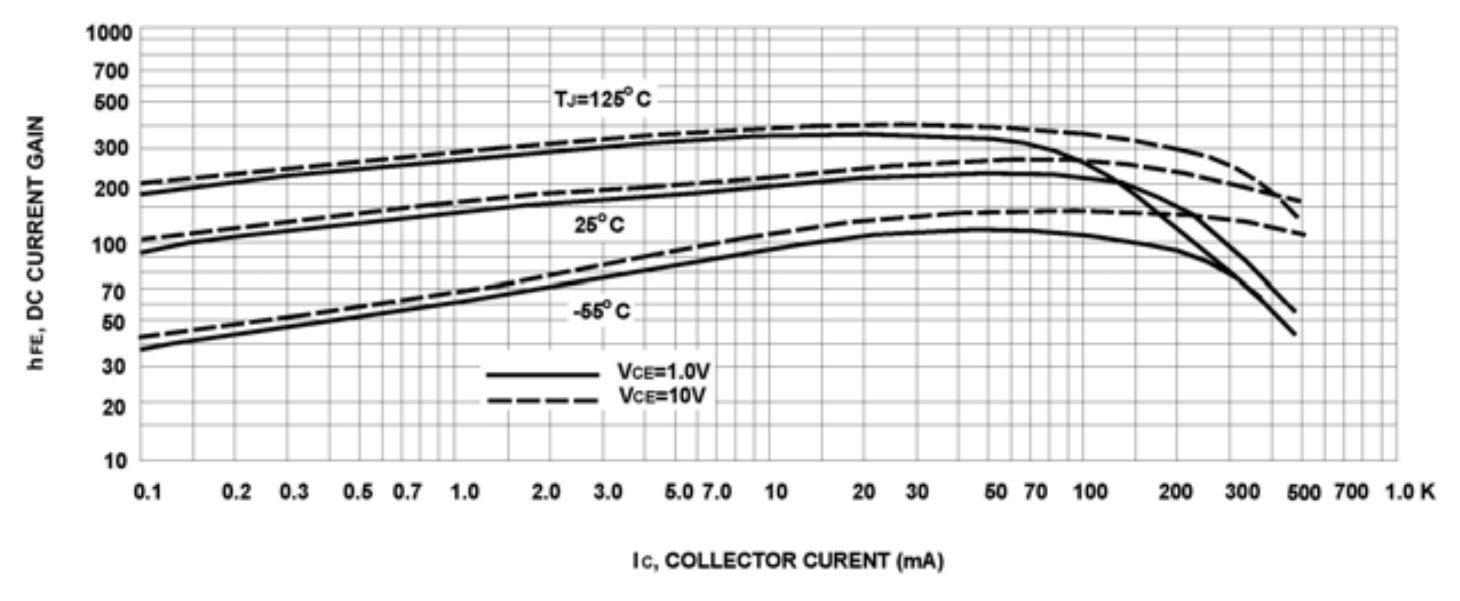
\includegraphics[width=1\linewidth]{chrome_Vv1MFWjHkn.png}
    
    \caption{Beta Values for Different Temperature Values}
    \label{fig:fig2}
\end{figure}

\begin{figure}[H]
    \centering
    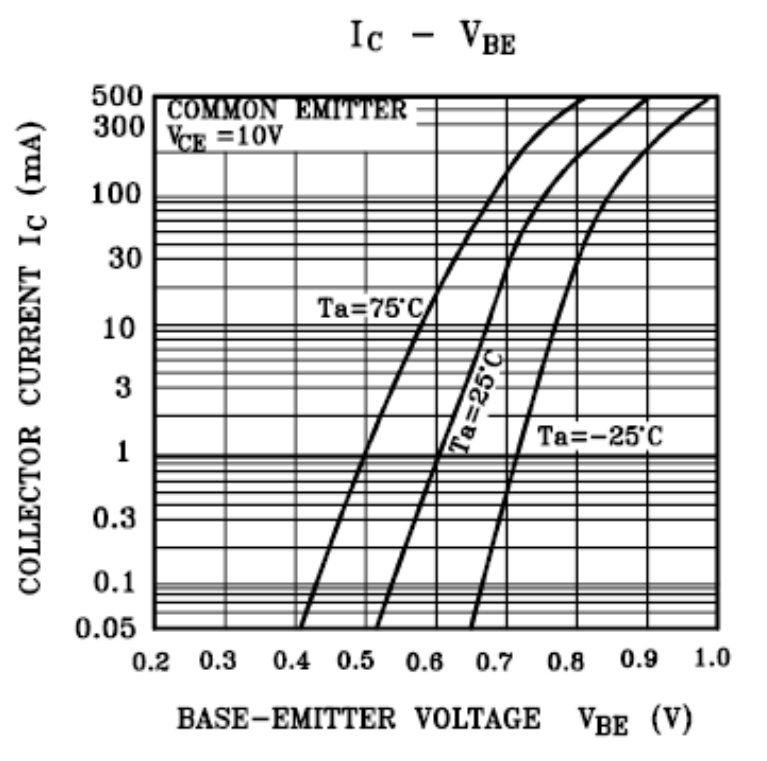
\includegraphics[width=0.5\linewidth]{chrome_wT6TTZ9f05.png}
        
    \caption{Relationship between the Collector Current and the Base-Emitter Voltage}
    \label{fig:fig3}
\end{figure}

\subsection{Circuit Design}

Summary of design parameters based on student ID (ending in $68$):
\begin{itemize}
    \item $f_{low} = 680$~Hz and $f_{high} = 13200$~Hz
    \item Target Gain: $8$ 
\end{itemize}

Calculations for each stage and schematics are given in \autoref{subsec:appendix_a}.

\subsubsection{Buffer Stage}

The following assumptions are made for this stage:
\[I_C=10~\mathrm{mA},\quad\beta=200,\quad V_{BE,~\text{ON}}=0.7~\text{V},\quad I_{R_1}\approx I_{R_2}\ge10~\mathrm{mA}.\]
The $\beta$ value is taken as $200$ by imposing the assumption $I_C=10$~mA for $T=25^\circ C$ from \autoref{fig:fig2}. By imposing the same assumption, the $V_{BE}$ value is taken as approximately $0.7$~V from \autoref{fig:fig3}. \autoref{tab:buffer_stage} lists the components for this stage.

\begin{table}[H]
\centering
\caption{Buffer Stage Component Values}
\begin{tabular}{|c|c|c|}
\hline
\textbf{Component} & \textbf{Value} & \textbf{Description} \\ \hline
$R_1$ & $6.8~\mathrm{k\Omega}$ & Base bias resistor (connected to DC) \\ \hline
$R_2$ & $10~\mathrm{k\Omega}$ & Base bias resistor (grounded)\\ \hline
$R_3$ & $470~\mathrm{\Omega}$ & Emitter resistor \\ \hline
$C_1$ & $1~\mathrm{\mu F}$ & Input coupling capacitor \\ \hline
$C_2$ & $10~\mathrm{\mu F}$ & Output coupling capacitor \\ \hline
$Q_1$ & 2N2222 & NPN BJT transistor \\ \hline
\end{tabular}
\label{tab:buffer_stage}
\end{table}

\subsubsection{Equalizer Stage}

~\autoref{tab:equalizer_stage} lists the components for this stage.

\begin{table}[H]
\centering
\caption{Equalizer Stage Component Values}
\begin{tabular}{|c|c|c|}
\hline
\textbf{Component} & \textbf{Value} & \textbf{Description} \\ \hline
$R_4$ & $1.2~\mathrm{k\Omega}$ & Low-pass resistor\\ \hline
$C_4$ & $10~\mathrm{nF}$ & Low-pass capacitor \\ \hline
$R_5$ & $24~\mathrm{k\Omega}$ & High-pass resistor\\ \hline
$C_5$ & $10~\mathrm{nF}$ & High-pass capacitor\\ \hline
\end{tabular}
\label{tab:equalizer_stage}
\end{table}


\subsubsection{Gain Stage}

Like the buffer stage, the following assumptions are made:
\[K = 0.085~\mathrm{A/V^2}\quad V_{DS} = 2 ~\mathrm{V},\quad V_{TH} = 1.6~\mathrm{mA},\quad I_{D,~\text{SAT}} = 2~\mathrm{mA}\]
~\autoref{tab:gain_stage} lists the components for this stage.

\begin{table}[H]
\centering
\caption{Gain Stage Component Values}
\begin{tabular}{|c|c|c|}
\hline
\textbf{Component} & \textbf{Value} & \textbf{Description} \\ \hline
$R_6$ & $560~\mathrm{k\Omega}$ & Gate bias resistor (connected to DC) \\ \hline
$R_7$ & $180~\mathrm{k\Omega}$ & Gate bias resistor (grounded)\\ \hline
$R_8$ & $2~\mathrm{k\Omega}$ & Collector resistor \\ \hline
$R_9$ & $220~\mathrm{\Omega}$ & Source resistor \\ \hline
$C_6$ & $1~\mathrm{\mu F}$ & Input coupling capacitor \\ \hline
$C_7$ & $10~\mathrm{\mu F}$ & Output coupling capacitor \\ \hline
$Q_2$ & 2N7000 & N-channel MOSFET transistor \\ \hline
\end{tabular}
\label{tab:gain_stage}
\end{table}

\subsection{Pros and Cons of Design}

BJTs provide relatively high transconductance and good voltage gain at low currents. However, in this circuit, the BJT is used as a buffer  based on preferences. The unbypassed emitter resistor improves thermal stability and linearity by introducing local negative feedback into the circuit.

The passive filters are highly predictable, stable, and very linear because there are no active semiconductor nonlinearities involved. They can be useful for AC coupling between stages or shaping the overall response of the circuit. The tradeoff is that passive networks always introduce attenuation, so some signal strength is lost.

One advantage of the MOSFET is the extremely high input impedance of the gate. Because there is essentially no gate current flowing, the input signal experiences little load. However, the gain may become less than the theoretical value compared to the one obtained with a BJT.

\section{Simulation}

The model 2N7000 didn't exist in the current LTspice environment. Therefore, a new spice directive \cite{4} is used. The directive for this model:

\texttt{.model 2N7000 VDMOS(Rg=3 Vto=1.6 Rd=0 Rs=.75 Rb=.14 Kp=.17}

\vspace{-1em}

\texttt{mtriode=1.25 Cgdmax=80p Cgdmin=12p Cgs=50p Cjo=50p Is=.04p}

\vspace{-1em}

\texttt{mfg=Fairchild Vds=60 Ron=2 Qg=1.5n)}

In each stage simulation, the directive \verb|.tran 0 2m 0 0.01m| is used and an input voltage of $20~\mathrm{mV}$ and the source frequency of $3~\mathrm{kHz}$, the approximate frequency transmitted the most, are assumed. At the buffer and gain stages, a measuring instrument with $1~\mathrm{M\Omega}$ internal resistance is assumed to be used to prevent the DC offset despite being not shown in the figures.

\subsection{Buffer Stage Simulation}

The stage design is given in \autoref{fig:buffer_stage_ltspice} and its simulation is given in \autoref{fig:buffer_stage_ltspice_sim}.

\begin{figure}[H]
    \centering
    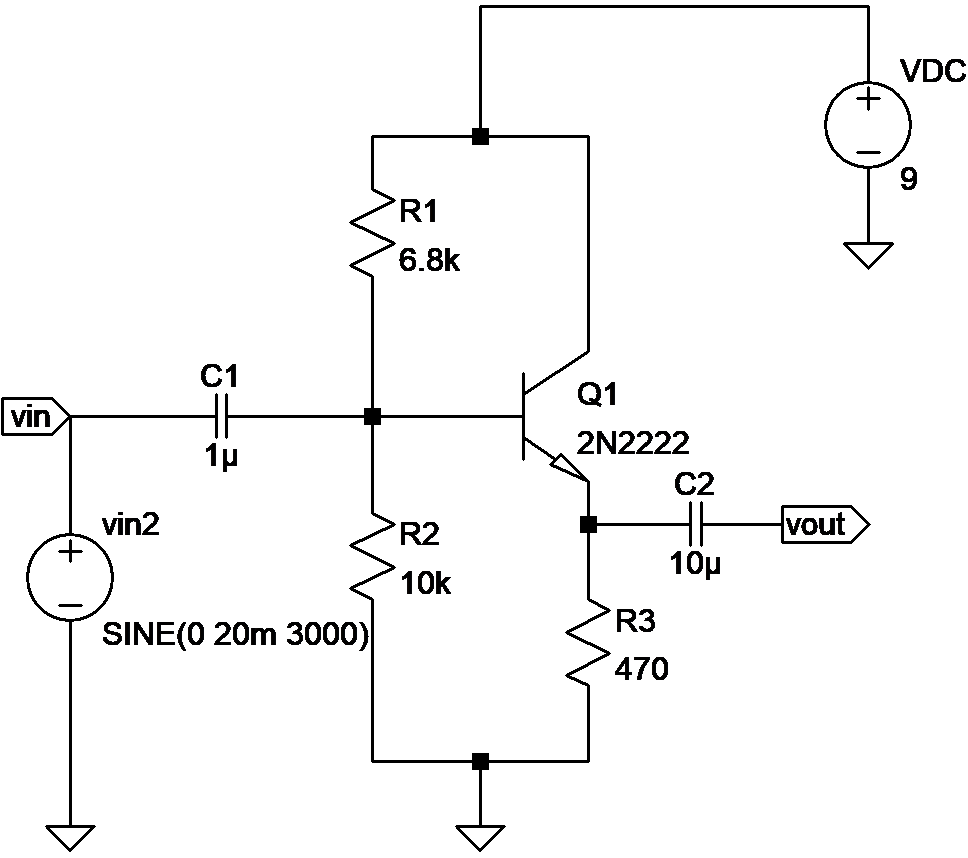
\includegraphics[width=0.75\linewidth]{buffer_stage_ltspice.png}

    \caption{Buffer Stage Simulation Circuit}
    \label{fig:buffer_stage_ltspice}
\end{figure}

\begin{figure}[H]
    \centering
    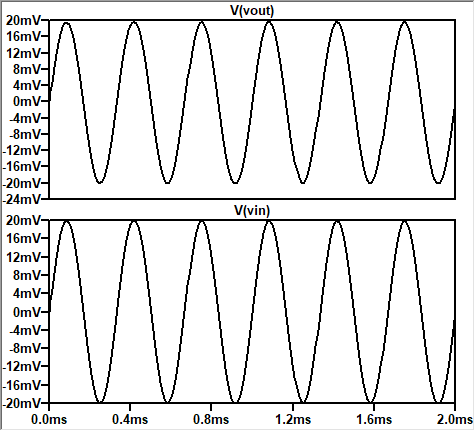
\includegraphics[width=0.65\linewidth]{buffer_stage_ltspice_sim.png}

    \caption{Buffer Stage Simulation}
    \label{fig:buffer_stage_ltspice_sim}
\end{figure}

As expected, the voltage gain is $A_v=1~\mathrm{V/V}$.

\subsection{Equalizer Stage Simulation}

The stage design is given in \autoref{fig:equalizer_stage_ltspice}.

\begin{figure}[H]
    \centering
    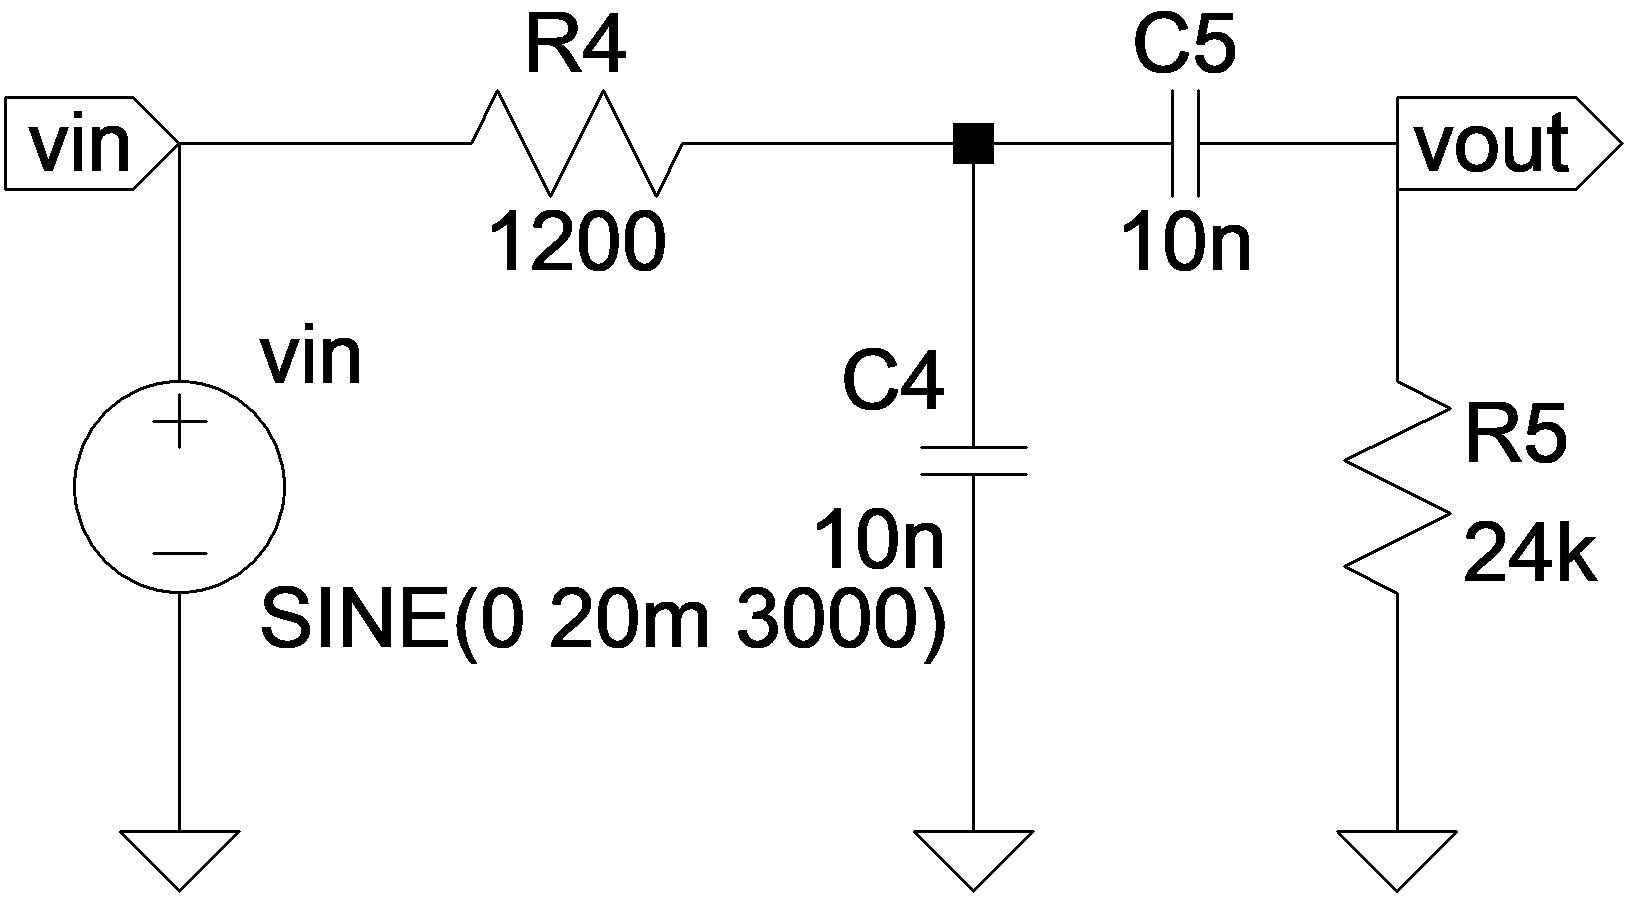
\includegraphics[width=0.65\linewidth]{equalizer_stage_ltspice.png}

    \caption{Equalizer Stage Simulation Circuit}
    \label{fig:equalizer_stage_ltspice}
\end{figure}

The input and output voltage are simulated in \autoref{fig:equalizer_stage_ltspice_sim1} and the amplitude of the output voltage is given in \autoref{fig:equalizer_stage_ltspice_sim1_comp}. 

\begin{minipage}{0.53\textwidth}
    \begin{figure}[H]
        \centering
        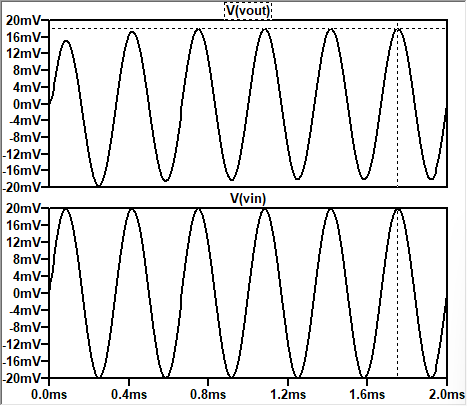
\includegraphics[width=1\linewidth]{equalizer_stage_ltspice_sim1.png}
        
    \caption{Equalizer Stage Simulation (Voltage Characteristics)}
    \label{fig:equalizer_stage_ltspice_sim1}
    \end{figure}
\end{minipage}\hfill\begin{minipage}{0.43\textwidth}
    \begin{figure}[H]
        \centering
        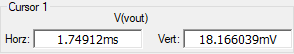
\includegraphics[width=1\linewidth]{equalizer_stage_ltspice_sim1_comp.png}
                
    \caption{Equalizer Stage Simulation (Voltage Characteristics) Comparison}
    \label{fig:equalizer_stage_ltspice_sim1_comp}
    \end{figure}

    For $f=3~\mathrm{kHz}$ and $V_{in}=20~\mathrm{mV}$, the input voltage is attenuated by approximately $9.8\%$. Therefore, we may infer that at least almost ten percent of the signal is attenuated for all frequency values.
\end{minipage}

\vspace{1em}

The Bode plot is given in \autoref{fig:equalizer_stage_ltspice_sim2} and the cutoff frequencies are given in \autoref{fig:equalizer_stage_ltspice_sim2_res}.

\begin{minipage}{0.53\textwidth}
    \begin{figure}[H]
        \centering
        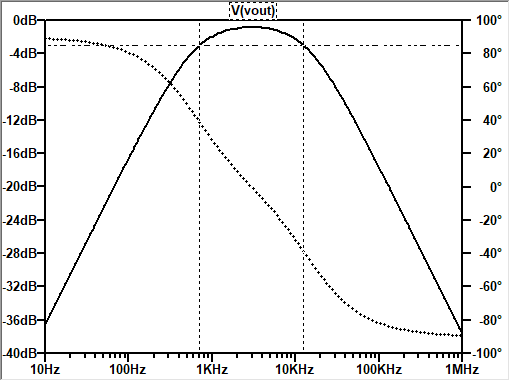
\includegraphics[width=1\linewidth]{equalizer_stage_ltspice_sim2.png}
        
    \caption{Equalizer Stage Simulation (Bode Plot)}
    \label{fig:equalizer_stage_ltspice_sim2}
    \end{figure}
\end{minipage}\hfill\begin{minipage}{0.43\textwidth}
    \begin{figure}[H]
        \centering
        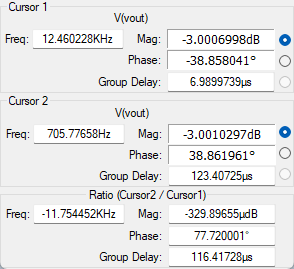
\includegraphics[width=1\linewidth]{equalizer_stage_ltspice_sim2_res.png}
                
    \caption{Equalizer Stage Simulation (Bode Plot) Result}
    \label{fig:equalizer_stage_ltspice_sim2_res}
    \end{figure}
\end{minipage}

The cutoff frequencies are found to be $f_{lower}\approx706~\mathrm{Hz}$ and $f_{upper}\approx12.460~\mathrm{kHz}$.

\newpage
\subsection{Gain Stage Simulation}

The stage design is given in \autoref{fig:gain_stage_ltspice} and its simulation is given in \autoref{fig:gain_stage_ltspice_sim}. The result is given in \autoref{fig:gain_stage_ltspice_sim_res}.

\begin{figure}[H]
    \centering
    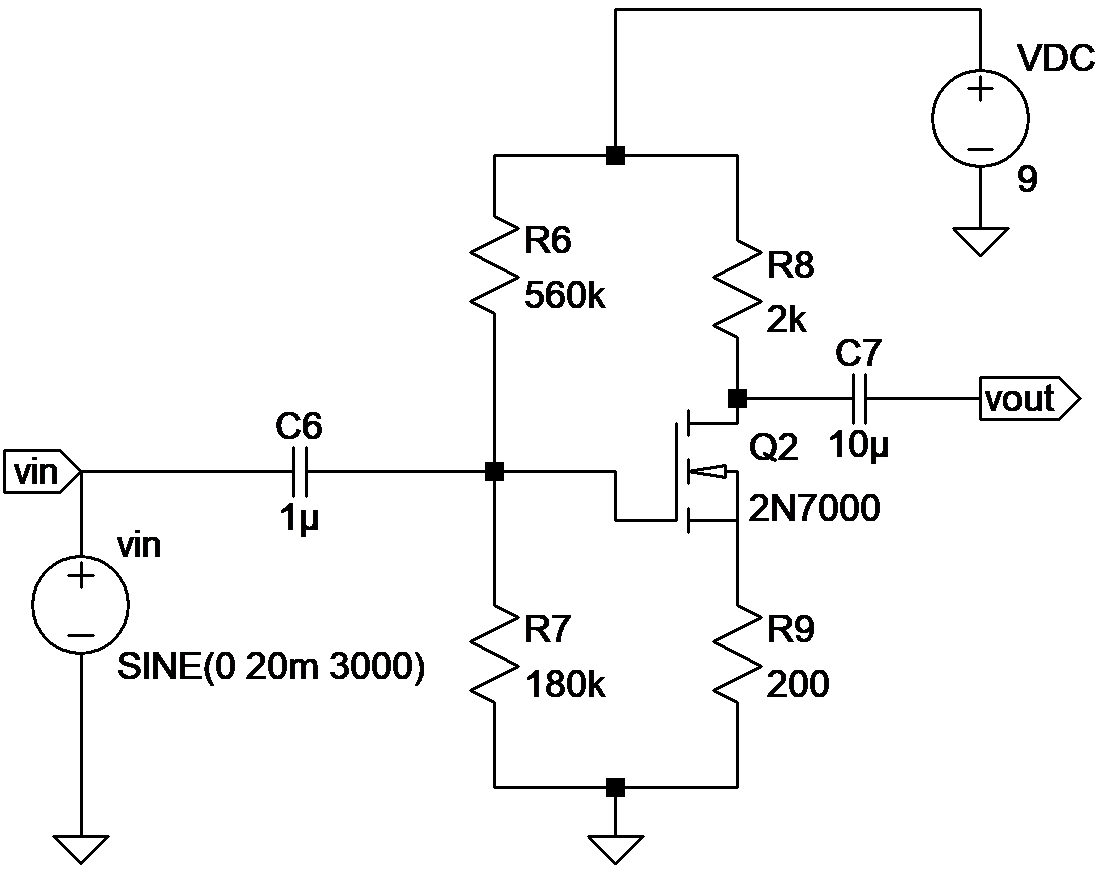
\includegraphics[width=0.75\linewidth]{gain_stage_ltspice.png}

    \caption{Gain Stage Simulation Circuit}
    \label{fig:gain_stage_ltspice}
\end{figure}


\begin{minipage}{0.53\textwidth}

\begin{figure}[H]
    \centering
    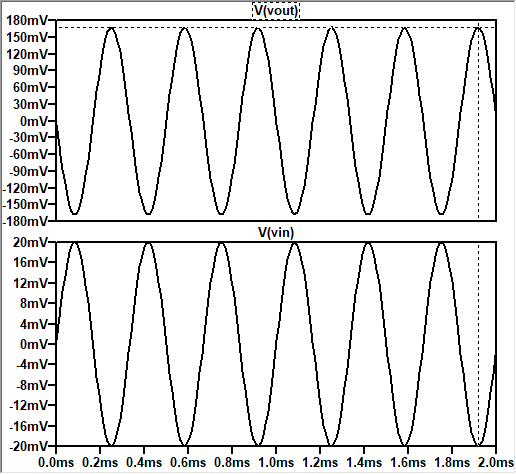
\includegraphics[width=1\linewidth]{gain_stage_ltspice_sim.png}

    \caption{Gain Stage Simulation}
    \label{fig:gain_stage_ltspice_sim}
\end{figure}
\end{minipage}\hfill\begin{minipage}{0.43\textwidth}

\begin{figure}[H]
    \centering
    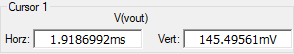
\includegraphics[width=1\linewidth]{full_stage_ltspice_sim_res.png}

    \caption{Gain Stage Simulation Result}
    \label{fig:full_stage_ltspice_sim_res}
\end{figure}

Thus the voltage gain is found to be $A_v\approx-8.38~\mathrm{V/V}$. As expected, there is a $180^\circ$ phase shift. The gain obtained from the simulation differs by a small amount from the desired value. 
\end{minipage}

\newpage
\subsection{Multistage Simulation}

The design is given in \autoref{fig:full_stage_ltspice} and its simulation is given in \autoref{fig:full_stage_ltspice_sim}. The result is given in \autoref{fig:full_stage_ltspice_sim_res}.

\begin{figure}[H]
    \centering
    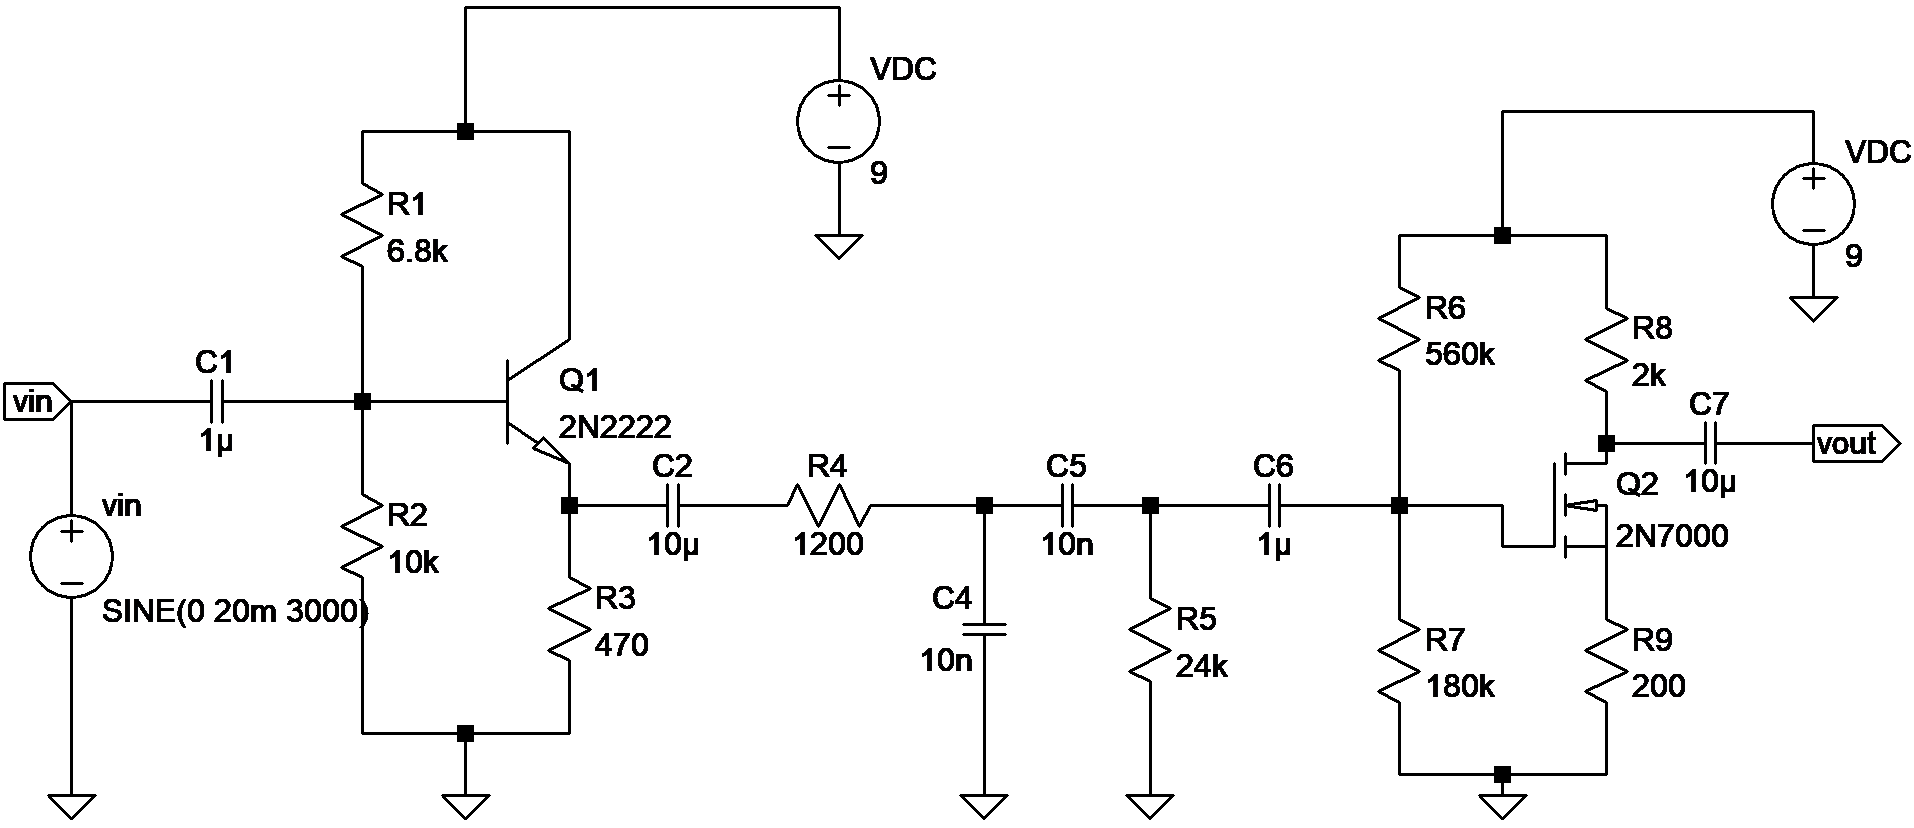
\includegraphics[width=1\linewidth]{full_stage_ltspice.png}

    \caption{Multistage Simulation Circuit}
    \label{fig:full_stage_ltspice}
\end{figure}


\begin{minipage}{0.53\textwidth}

\begin{figure}[H]
    \centering
    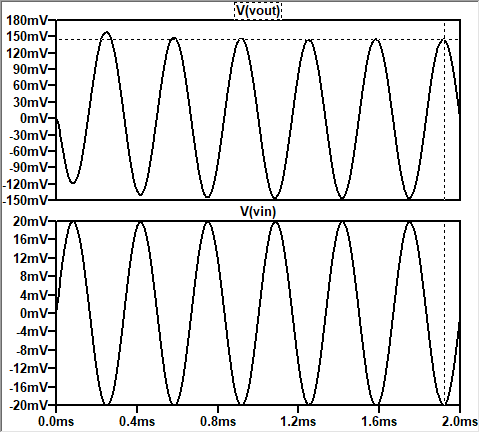
\includegraphics[width=1\linewidth]{full_stage_ltspice_sim.png}

    \caption{Multistage Simulation}
    \label{fig:full_stage_ltspice_sim}
\end{figure}
\end{minipage}\hfill\begin{minipage}{0.43\textwidth}

\begin{figure}[H]
    \centering
    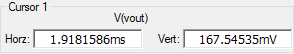
\includegraphics[width=1\linewidth]{gain_stage_ltspice_sim_res.png}

    \caption{Multistage Simulation Result}
    \label{fig:gain_stage_ltspice_sim_res}
\end{figure}

Thus the overall voltage gain is found to be $A_v\approx-7.27~\mathrm{V/V}$. As expected, there is a $180^\circ$ phase shift. The overall voltage gain obtained from the simulation differs by $1.11$ from the gain stage output gain and $0.73$ from the desired value in magnitude.
\end{minipage}

\section{Fabrication}

The circuit components were purchased from the shopkeepers on Konya Street. Since it would take some time to form up a brand new PCB, we decided to use a pertinax to solder and assemble the components. Before that, the circuit is tested on a breadboard to ensure that it is operating as expected. Timestamps of photos are given in \autoref{subsec:appendix_b}.

\subsection{Breadboard Testing}

\autoref{fig:buffer_stage_breadboard} shows the assembly of the buffer stage on the breadboard and \autoref{fig:buffer_stage_breadboard_meas} demonstrates whether the buffer stage works properly.

\begin{minipage}[t]{0.36\textwidth}
\vspace{0pt}
\centering
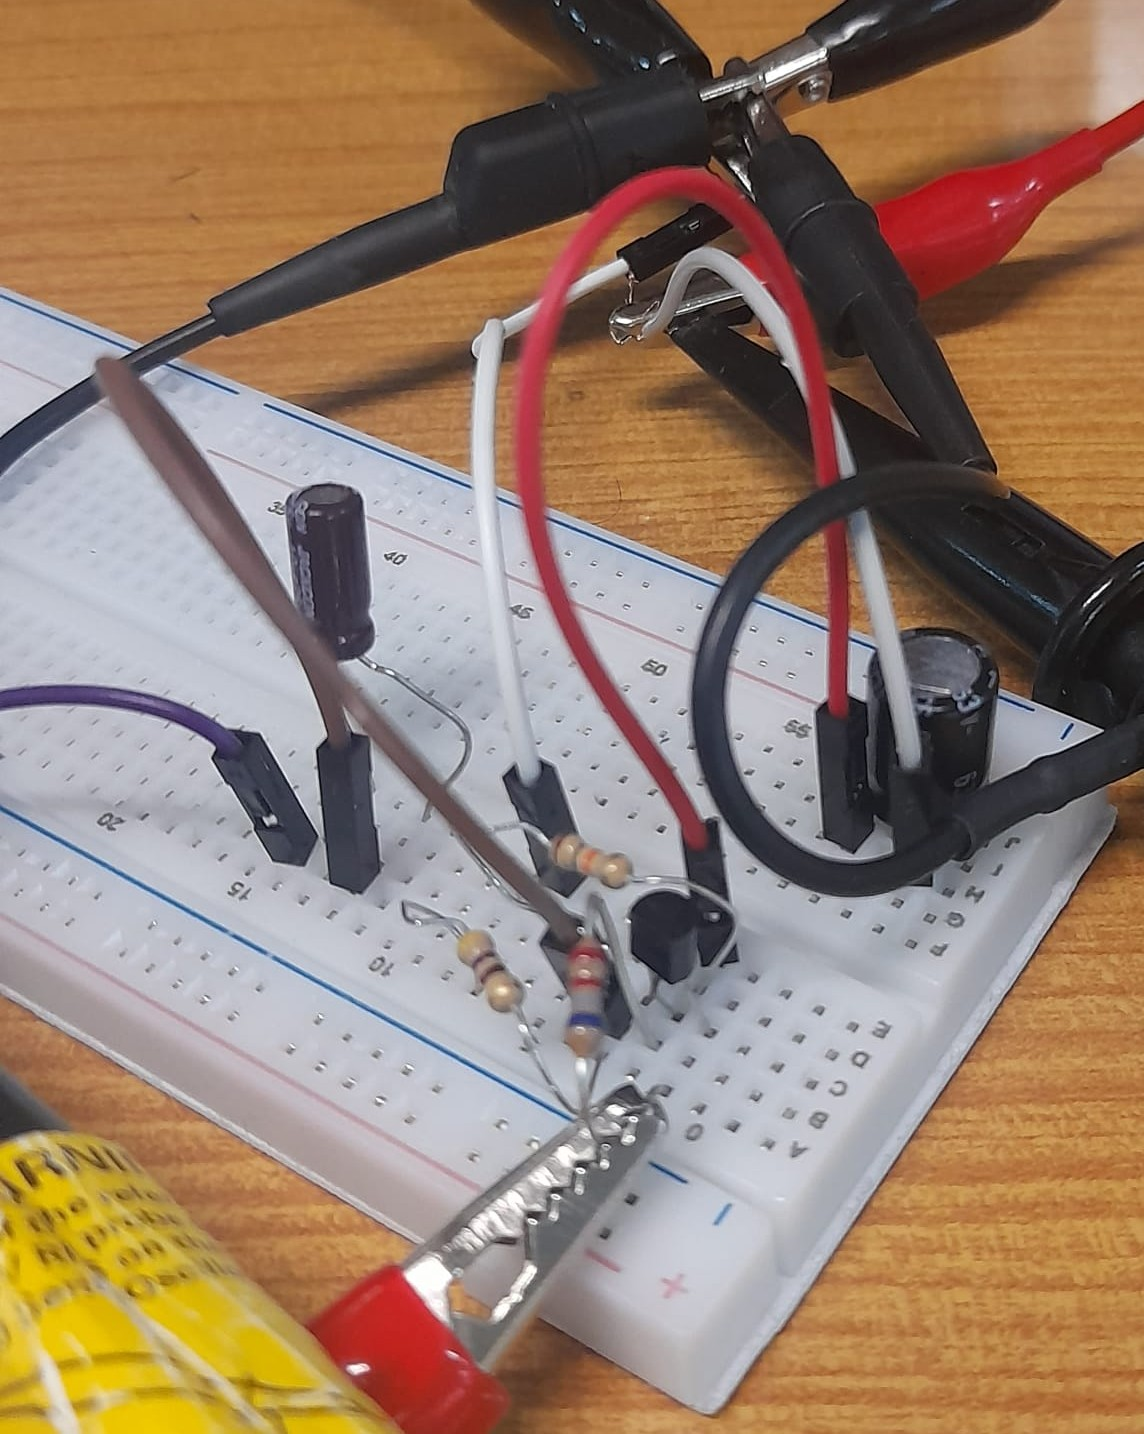
\includegraphics[width=\linewidth]{buffer_stage_breadboard_c1.jpeg}
\captionof{figure}{Buffer Stage on the Breadboard}
\label{fig:buffer_stage_breadboard}
\end{minipage}
\hfill
\begin{minipage}[t]{0.6\textwidth}
\vspace{0pt}
\centering
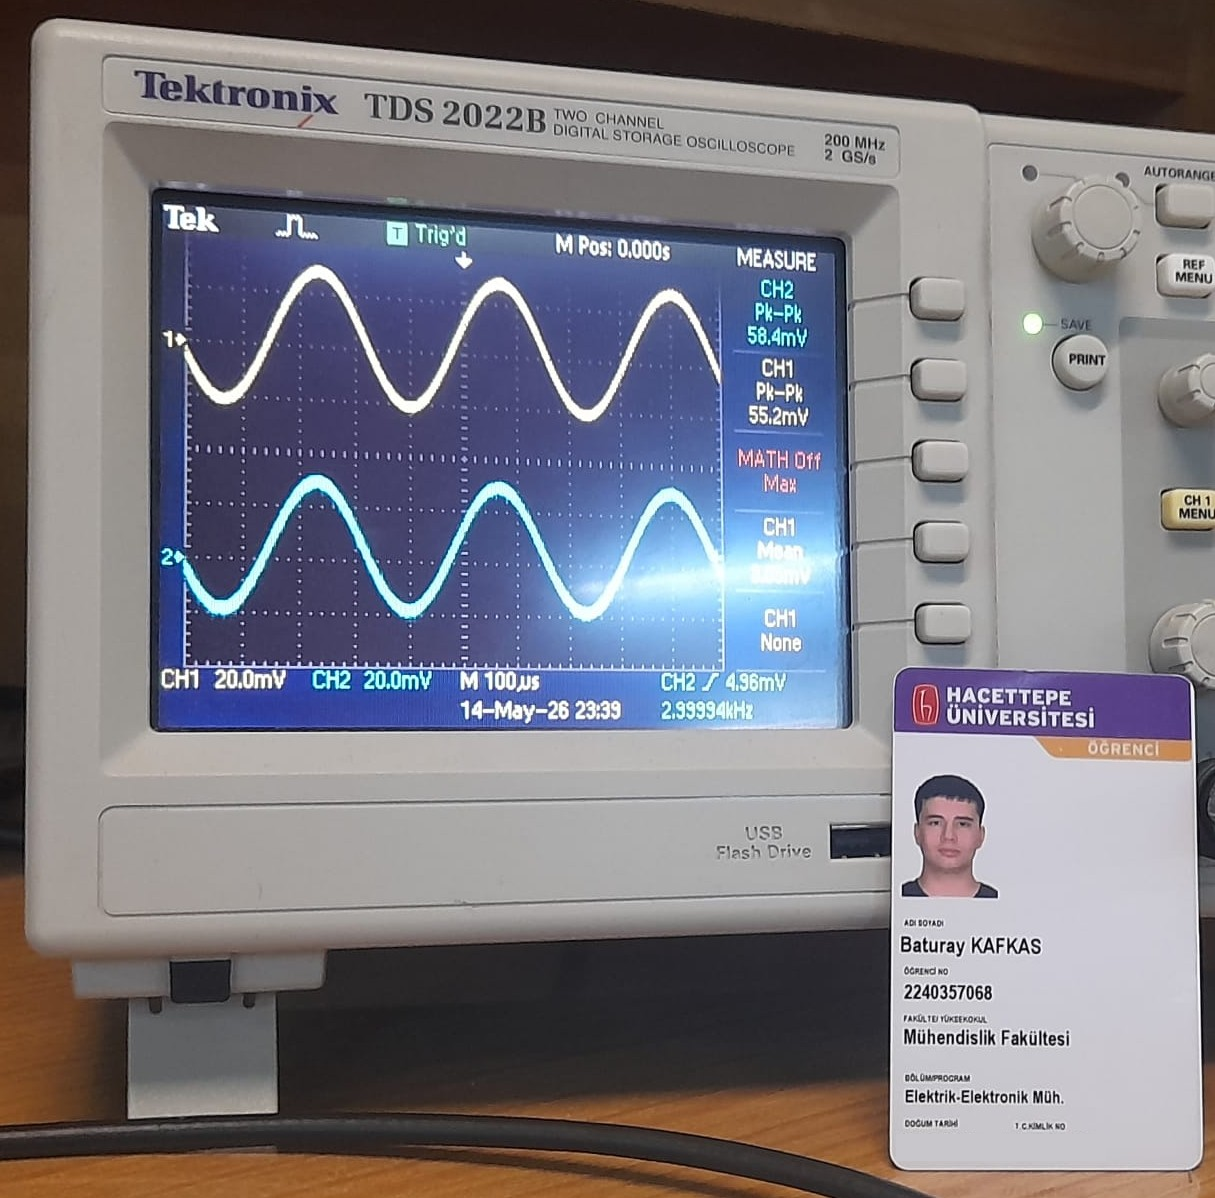
\includegraphics[width=\linewidth]{buffer_stage_breadboard_meas_c1.png}
\captionof{figure}{Output Voltage of the Buffer Stage on the Breadboard}
\label{fig:buffer_stage_breadboard_meas}
\end{minipage}

For $V_{in}$ set to $50~\mathrm{mV_{pp}}$, the input and output voltages are measured to be $55.2~\mathrm{mV}$ and $58.4~\mathrm{mV}$, respectively, indicating a healthy buffer stage with a negligible difference.

\autoref{fig:equalizer_stage_breadboard} shows the assembly of the gain stage on the breadboard and \autoref{fig:equalizer_stage_breadboard_meas1} and \autoref{fig:equalizer_stage_breadboard_meas2} demonstrate whether the gain stage works properly.

\begin{figure}[H]
    \centering
    \includegraphics[width=0.6\linewidth]{equalizer_stage_breadboard_C1.jpeg}
        
    \caption{Equalizer Stage on the Breadboard}
    \label{fig:equalizer_stage_breadboard}
\end{figure}

\begin{figure}[H]
    \centering
    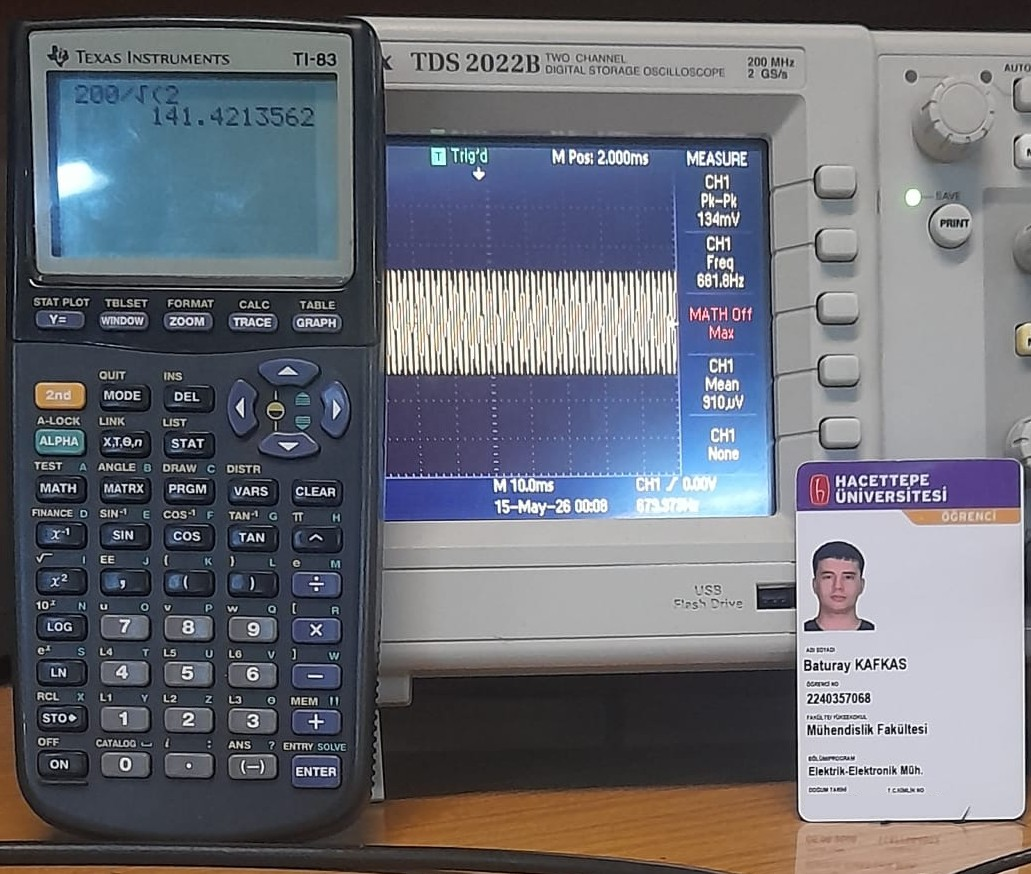
\includegraphics[width=0.68\linewidth]{equalizer_stage_breadboard_meas1_c1.png}
        
    \caption{Equalizer Stage on the Breadboard Adjusted for Lower Cutoff Frequency}
    \label{fig:equalizer_stage_breadboard_meas1}
\end{figure}

\begin{figure}[H]
    \centering
    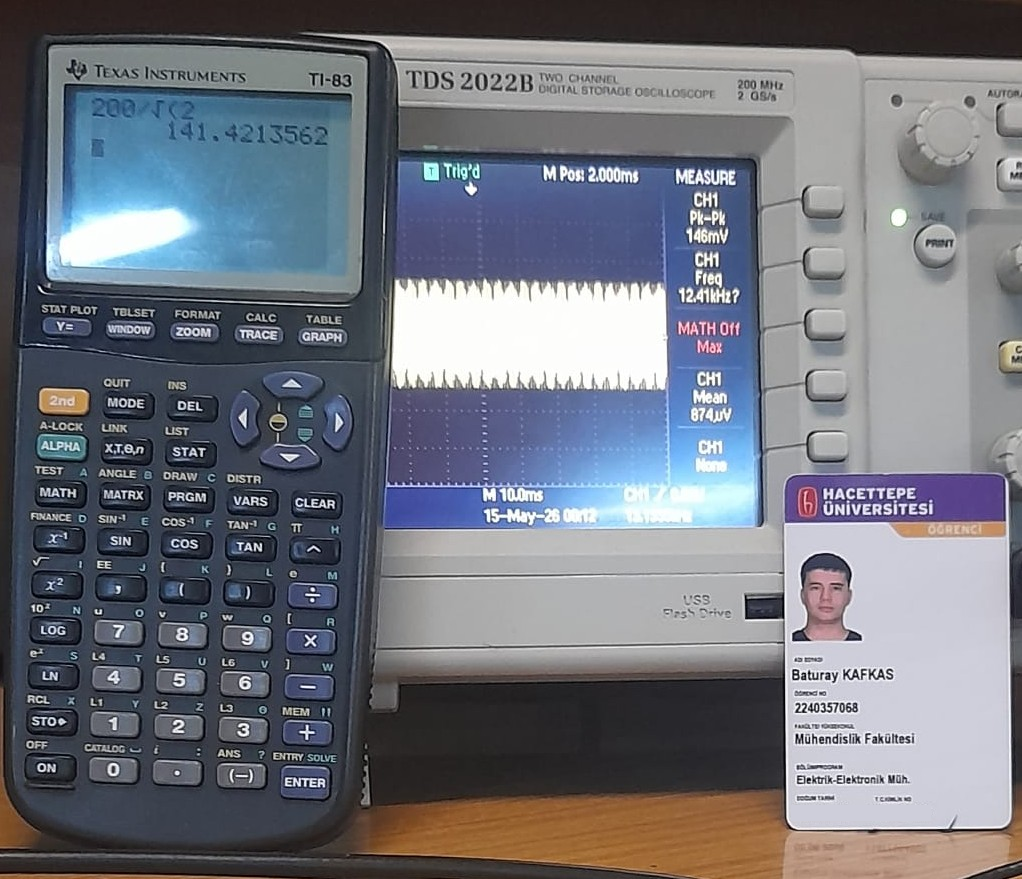
\includegraphics[width=0.68\linewidth]{equalizer_stage_breadboard_meas2_c1.png}
        
    \caption{Equalizer Stage on the Breadboard Adjusted for Upper Cutoff Frequency}
    \label{fig:equalizer_stage_breadboard_meas2}
\end{figure}

As seen above, the equalizer stage also works fine. The half of the power is consumed when these frequencies are applied.

\autoref{fig:gain_stage_breadboard} shows the assembly of the gain stage on the breadboard and \autoref{fig:gain_stage_breadboard_meas} demonstrates whether the gain stage works properly. \autoref{fig:multistage_breadboard_and_results} shows the assembly of the multistage amplifier on the breadboard and the results.


\begin{minipage}[t]{0.42\textwidth}
\vspace{0pt}
{
\centering
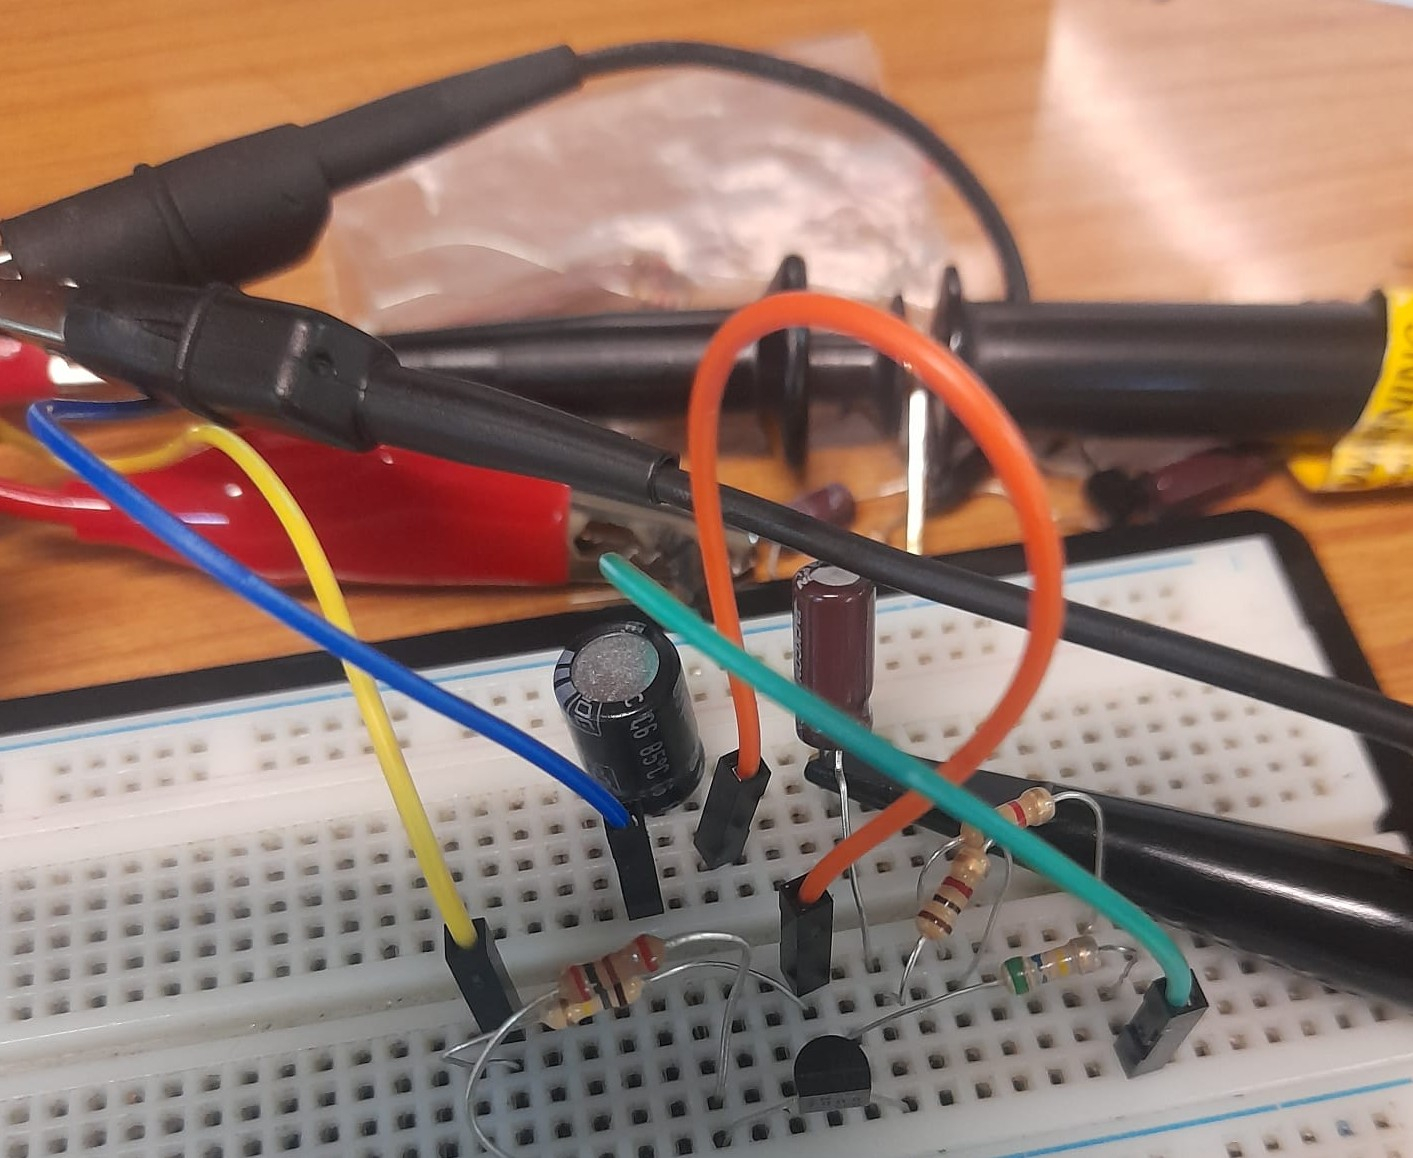
\includegraphics[width=\linewidth]{gain_stage_breadboard_c1.jpeg}
\captionof{figure}{Gain Stage on the Breadboard}
\label{fig:gain_stage_breadboard}
}
\vspace{1em}

The gain obtained in this stage is 
\[A_v=-408/54.4~\mathrm{V/V}=-7.5~\mathrm{V/V},\]
which is quite reasonable.

\end{minipage}
\hfill
\begin{minipage}[t]{0.54\textwidth}
\vspace{0pt}
\centering
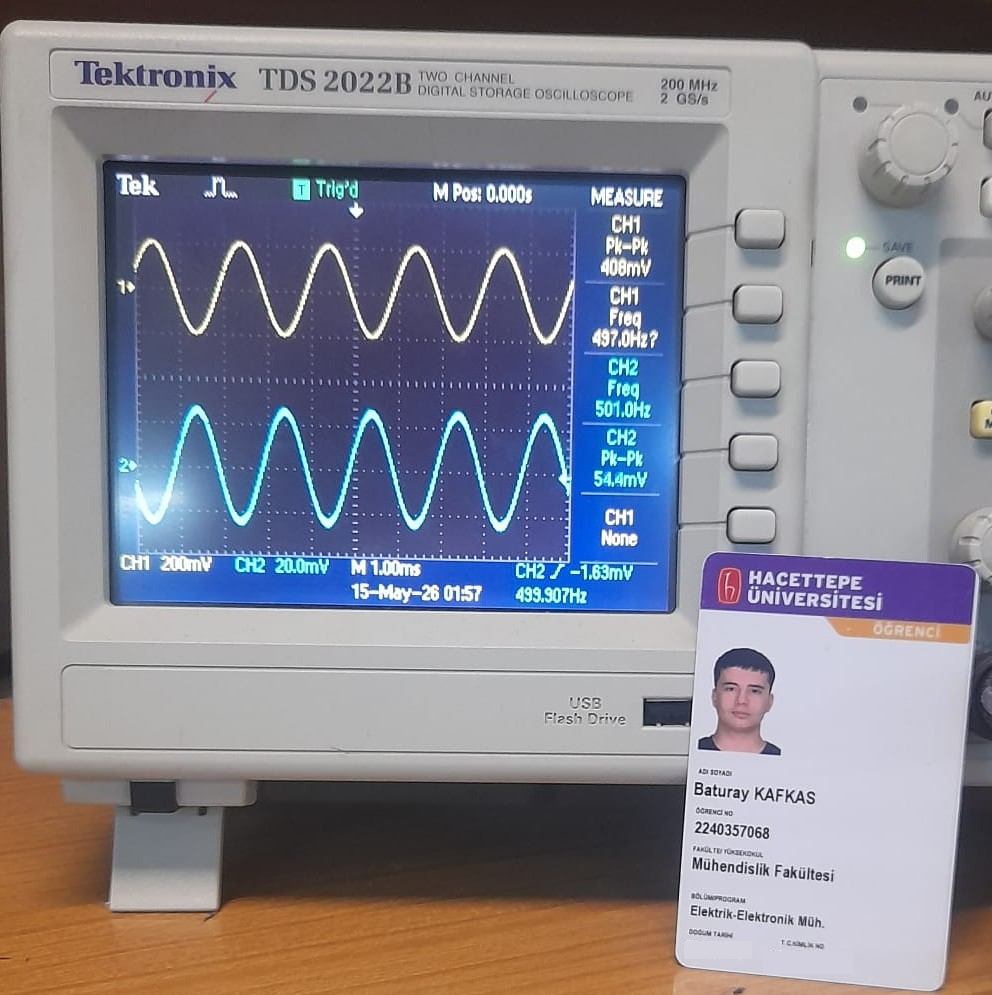
\includegraphics[width=\linewidth]{gain_stage_breadboard_meas_c1.png}
\captionof{figure}{Output Voltage of the Gain Stage on the Breadboard}
\label{fig:gain_stage_breadboard_meas}
\end{minipage}

\begin{comment}
\begin{minipage}[t]{0.48\textwidth}
\vspace{0pt}
\centering
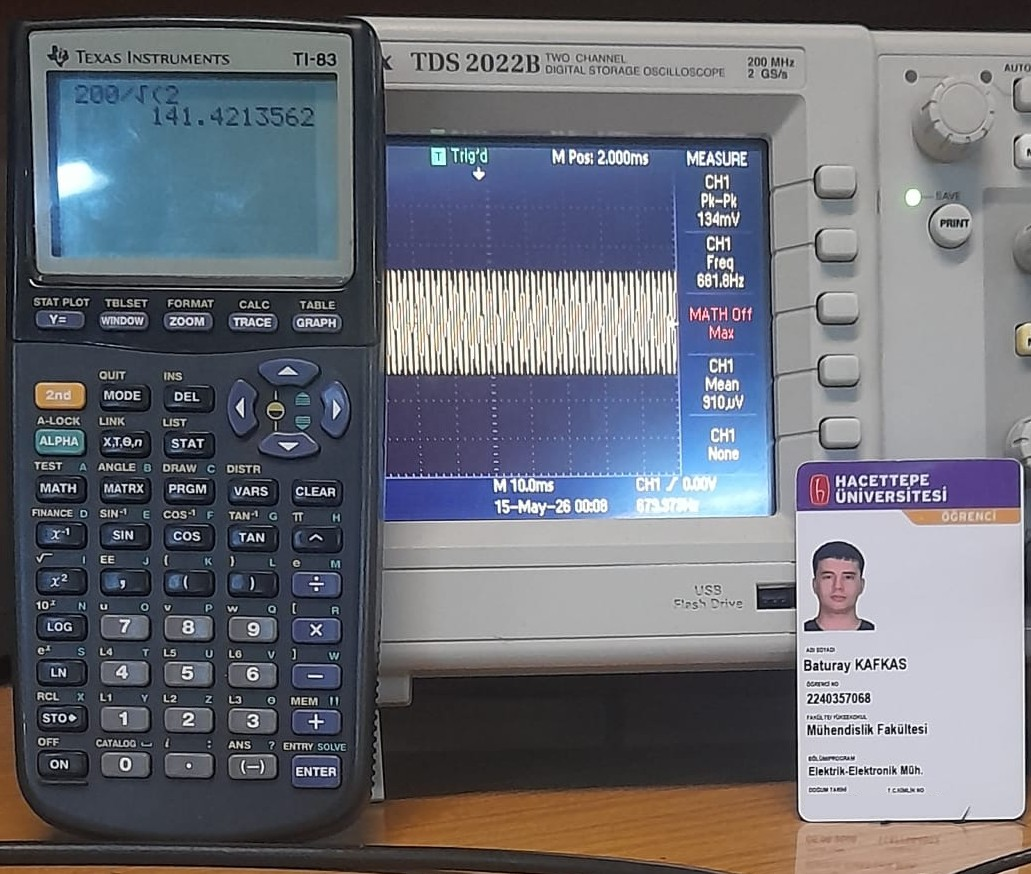
\includegraphics[width=\linewidth]{equalizer_stage_breadboard_meas1_c1.jpeg}
\captionof{figure}{Equalizer Stage on the Breadboard with }
\label{fig:equalizer_stage_breadboard_meas1}
\end{minipage}
\hfill
\begin{minipage}[t]{0.48\textwidth}
\vspace{0pt}
\centering
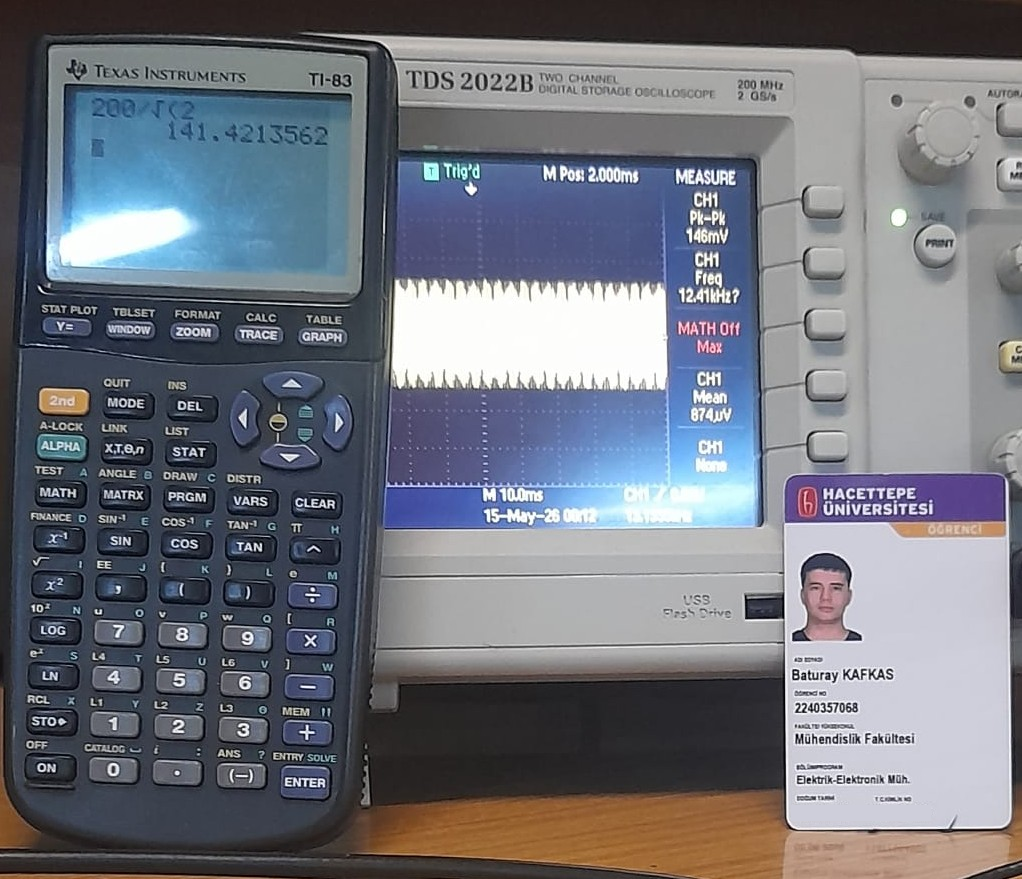
\includegraphics[width=\linewidth]{equalizer_stage_breadboard_meas2_c1.jpeg}
\captionof{figure}{Voltage Output of the Equalizer Stage on the Breadboard}
\label{fig:equalizer_stage_breadboard_meas2}
\end{minipage}
\end{comment}

\begin{figure}[H]
    \centering
    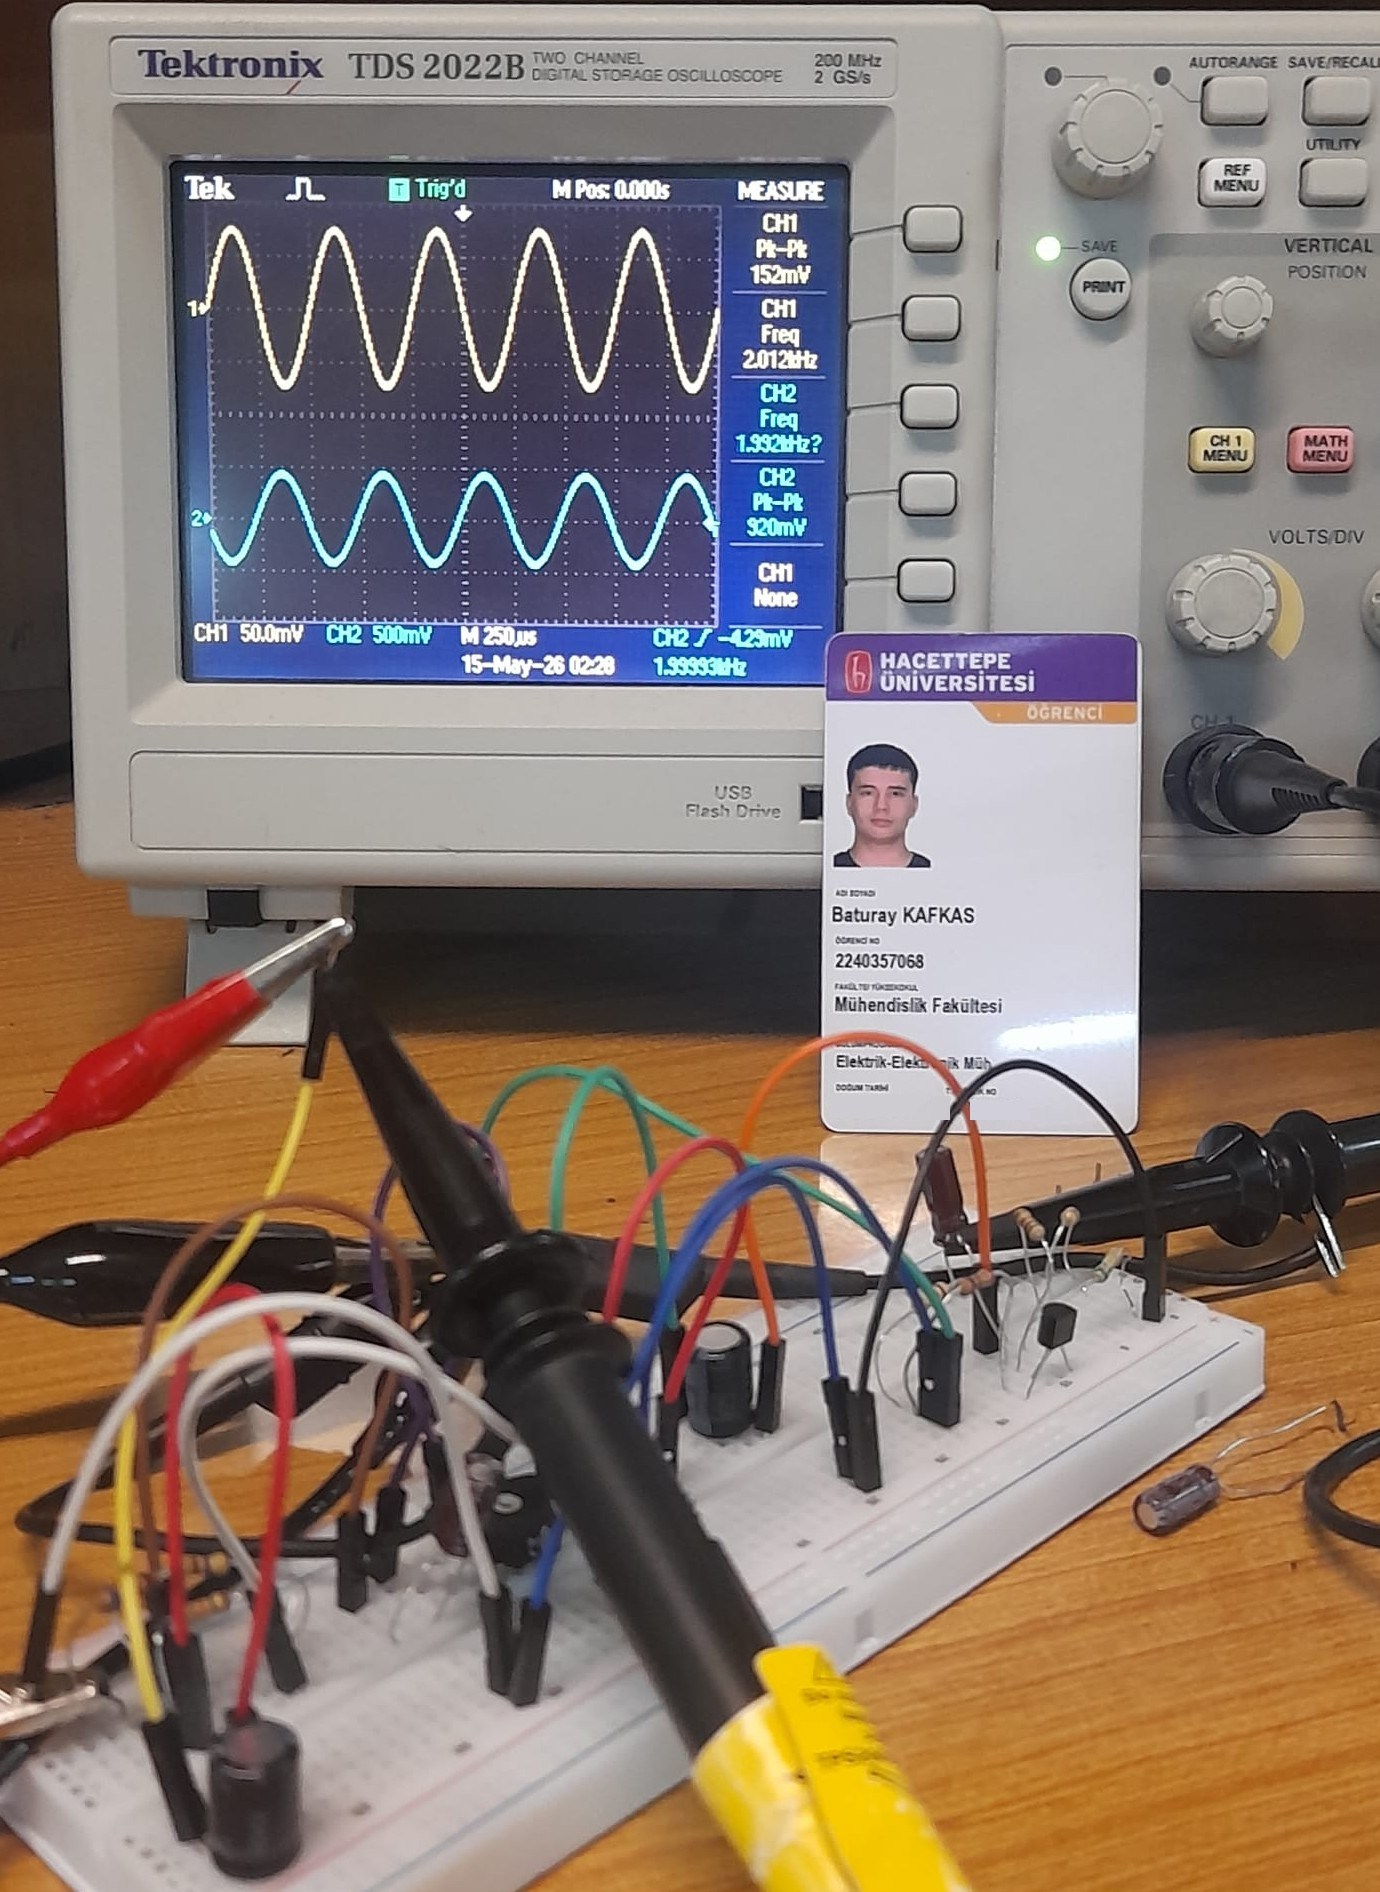
\includegraphics[width=0.54\linewidth]{multistage_breadboard_and_results_c1.jpg}

    \caption{Multistage Audio Amplifier on the Breadboard and its Testing}    \label{fig:multistage_breadboard_and_results}
\end{figure}

The overall gain is measured to be $A_v=-920/152~\mathrm{V/V}\approx-6.05$, indicating a $25\%$ loss.

\autoref{fig:breadboard_debugging} and \autoref{fig:breadboard_testing} demonstrate the process of building the circuit on the breadboard.

\begin{minipage}[t]{0.48\textwidth}
\vspace{0pt}
{
\centering
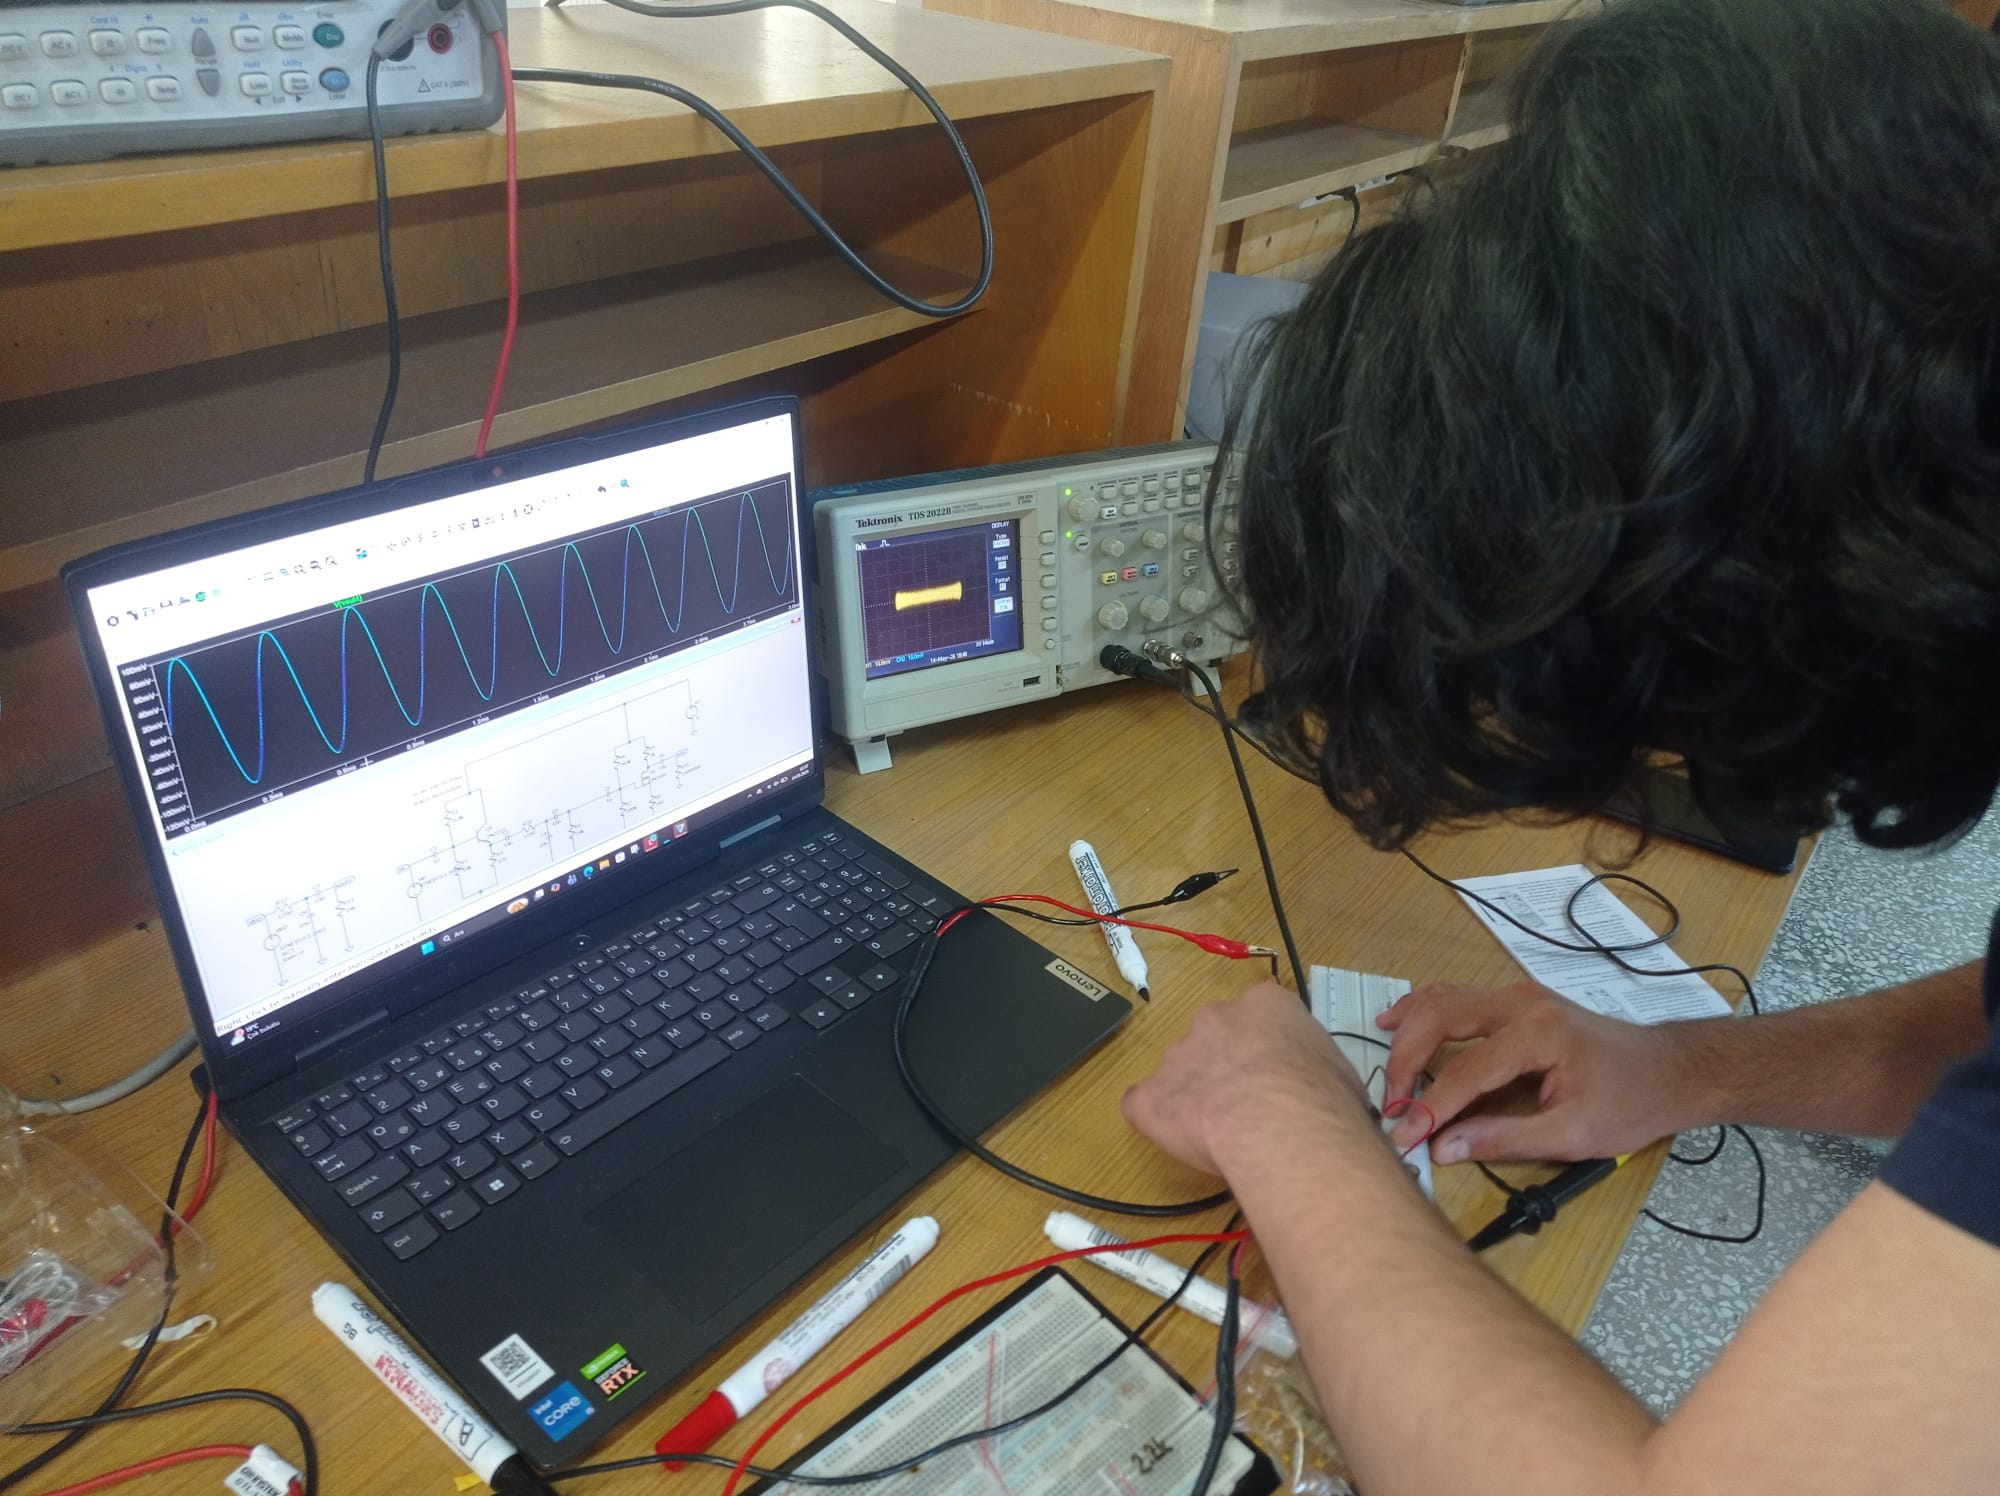
\includegraphics[width=\linewidth]{breadboard_debugging.jpeg}
\captionof{figure}{Breadboard Debugging}
\label{fig:breadboard_debugging}
}
\vspace{1em}

\end{minipage}
\hfill
\begin{minipage}[t]{0.48\textwidth}
\vspace{0pt}
\centering
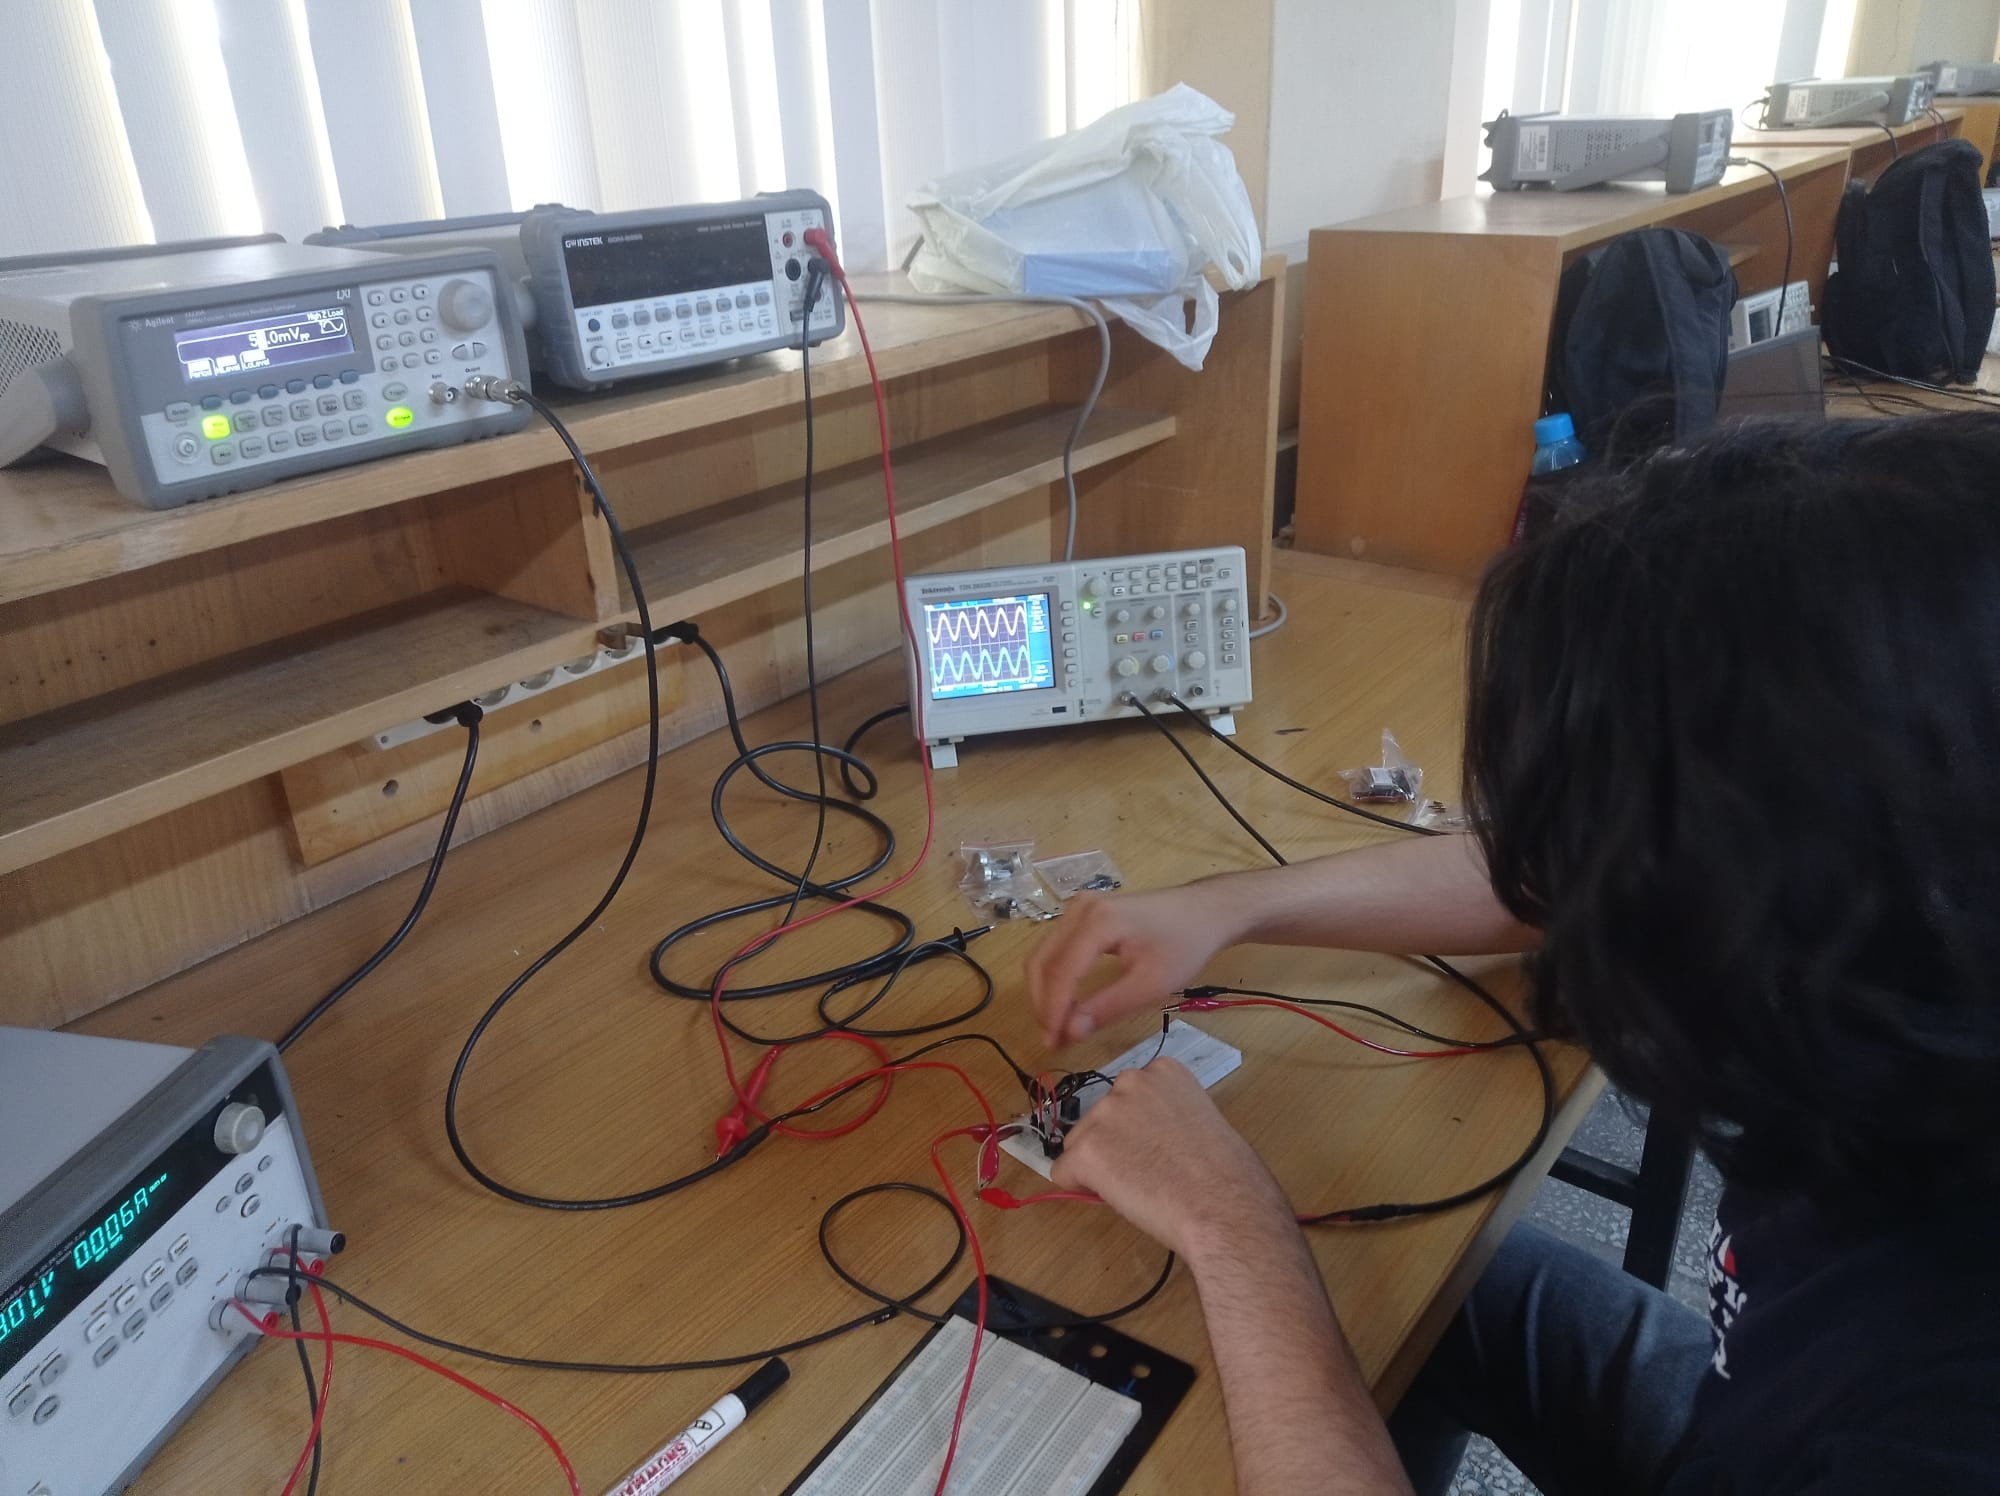
\includegraphics[width=\linewidth]{breadboard_testing.jpeg}
\captionof{figure}{Breadboard Testing}
\label{fig:breadboard_testing}
\end{minipage}

\subsection{Assembly on Pertinax}

From the simulation and breadboard testing, we can conclude that the gain is most likely to be lower than the desired value. Therefore, we decided to add a series potentiometer to the drain line in order to adjust the gain.

\begin{minipage}[t]{0.38\textwidth}
\vspace{0pt}
{
\centering
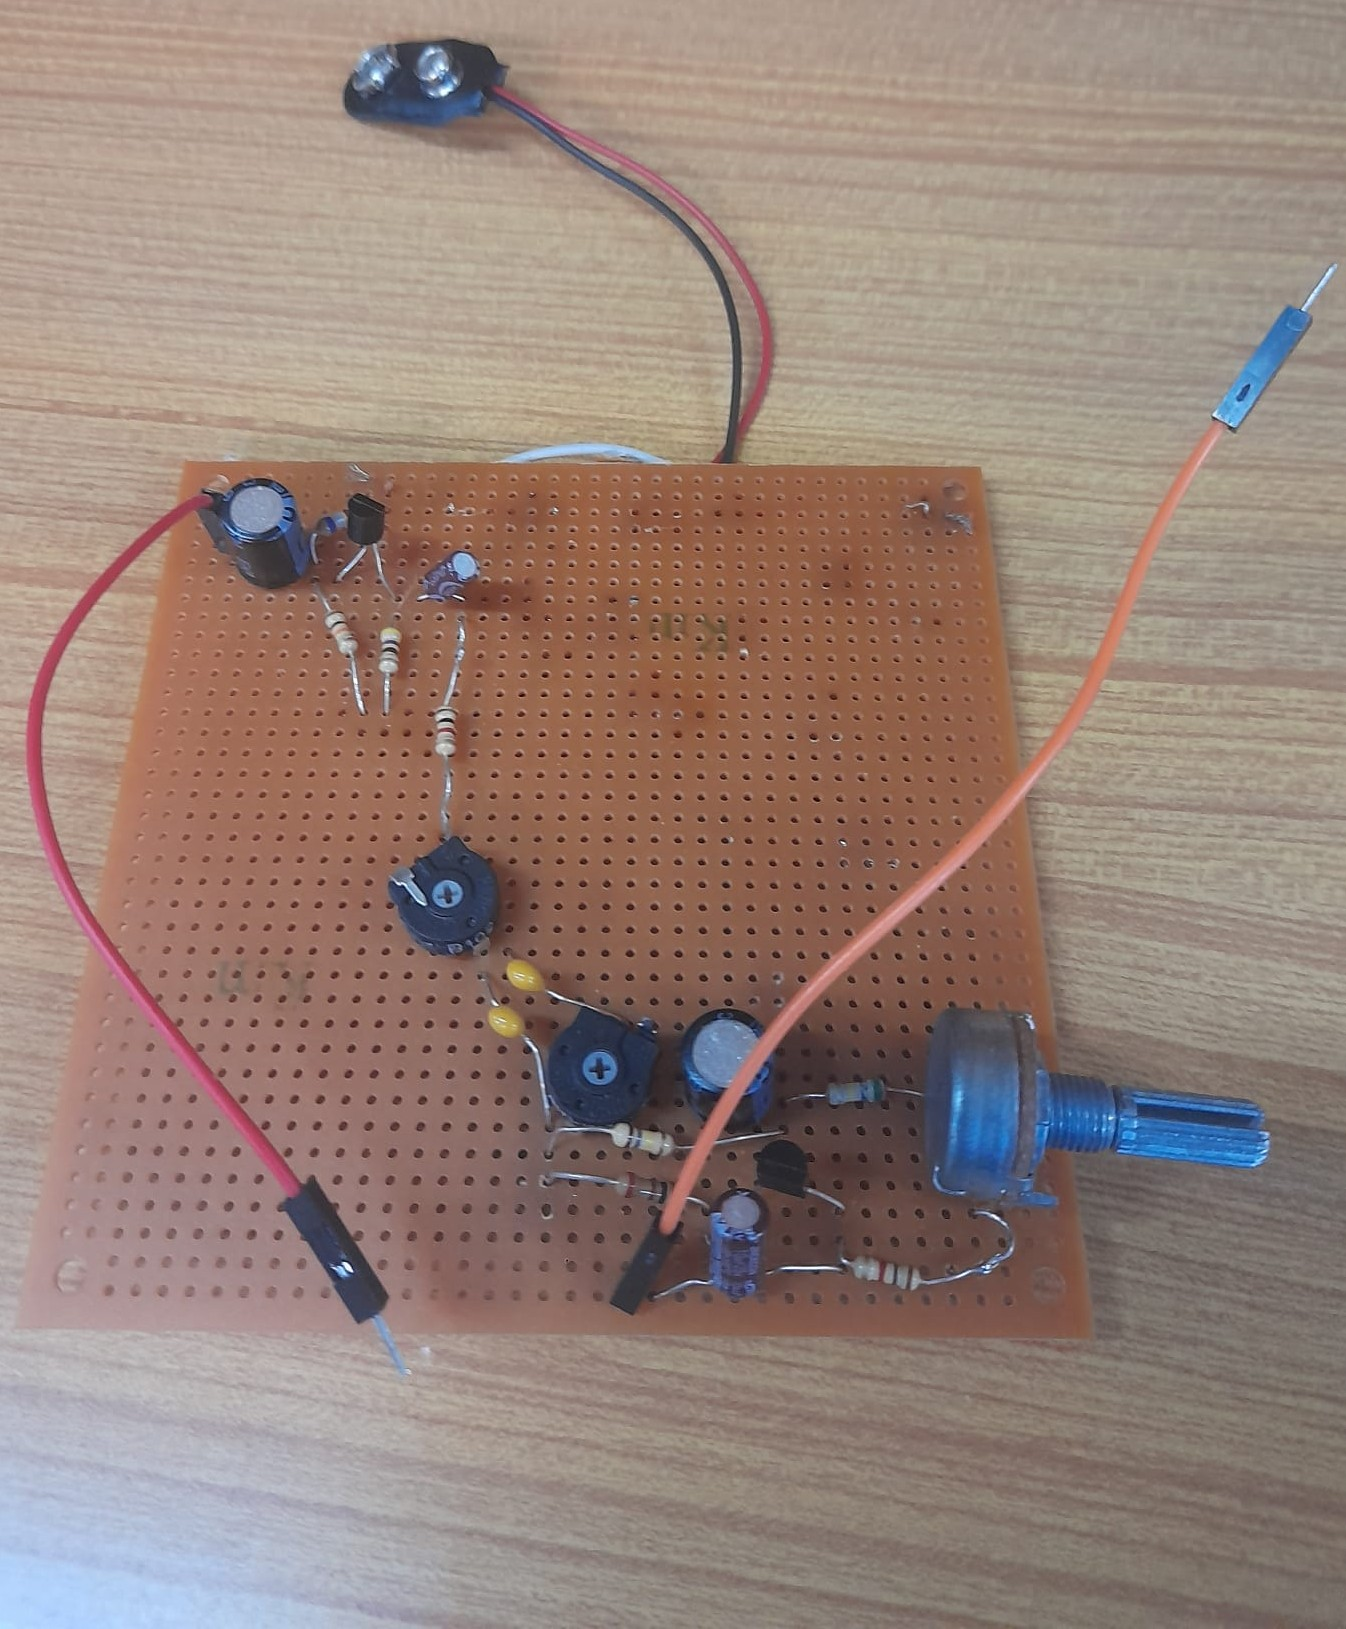
\includegraphics[width=\linewidth]{pertinax_circuit_c1.jpeg}
\captionof{figure}{Circuit Fabricated on a Pertinax}
\label{fig:pertinax_circuit}
}
\vspace{1em}

\end{minipage}
\hfill
\begin{minipage}[t]{0.58\textwidth}
\vspace{0pt}
\centering
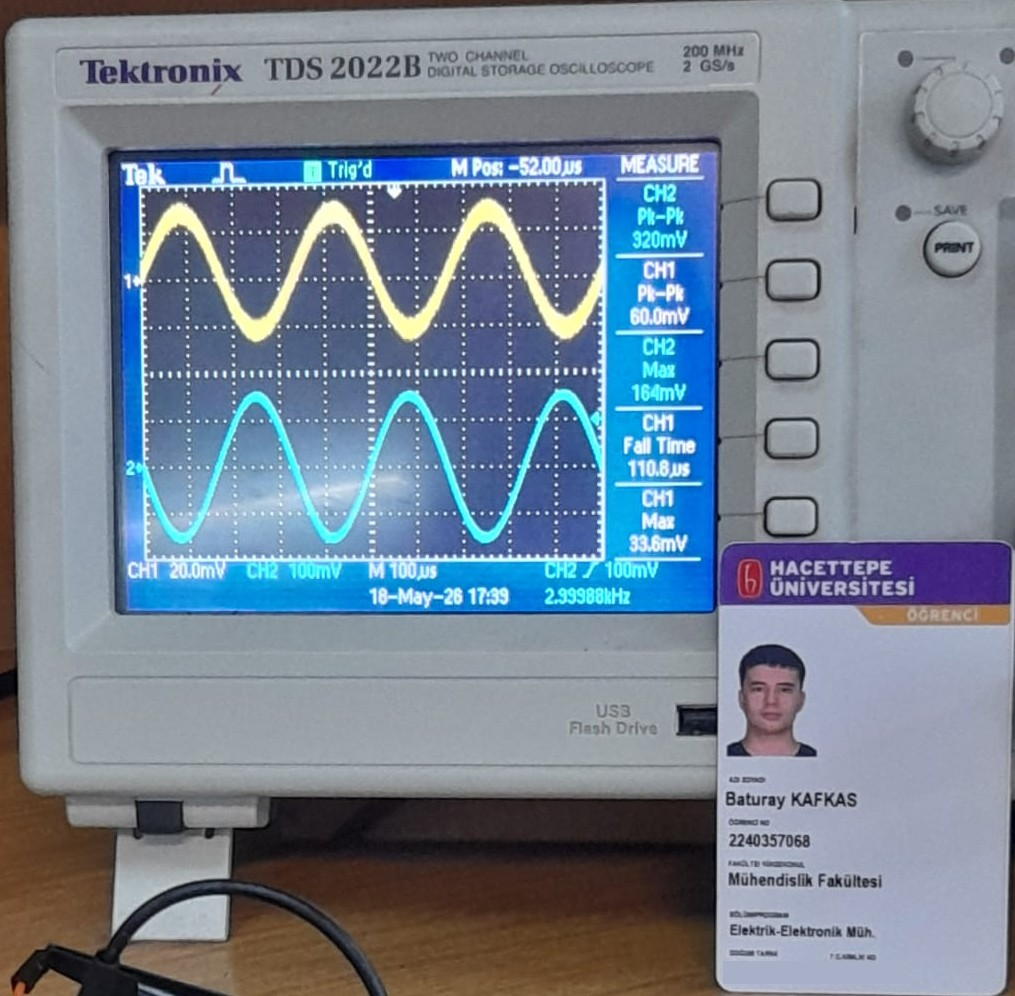
\includegraphics[width=\linewidth]{pertinax_circuit_meas1_c1.png}
\captionof{figure}{Testing of the Circuit Fabricated on a Pertinax}
\label{fig:pertinax_circuit_meas1}
\end{minipage}

For an input voltage of $50~\mathrm{mV_{pp}}$, the gain is $A_v=-320/60.0~\mathrm{V/V}\approx-5.33~\mathrm{V/V}$. If the first channel had measured $50~\mathrm{mV_{pp}}$, we would obtain $A_v=-320/50~\mathrm{V/V}=-6.4~\mathrm{V/V}$.

\autoref{fig:pertinax_circuit_meas2} and \autoref{fig:pertinax_circuit_meas3} show the minimum and maximum gain that can be obtained with the introduction of the potentiometer, respectively.

\begin{minipage}[t]{0.48\textwidth}
\vspace{0pt}
{
\centering
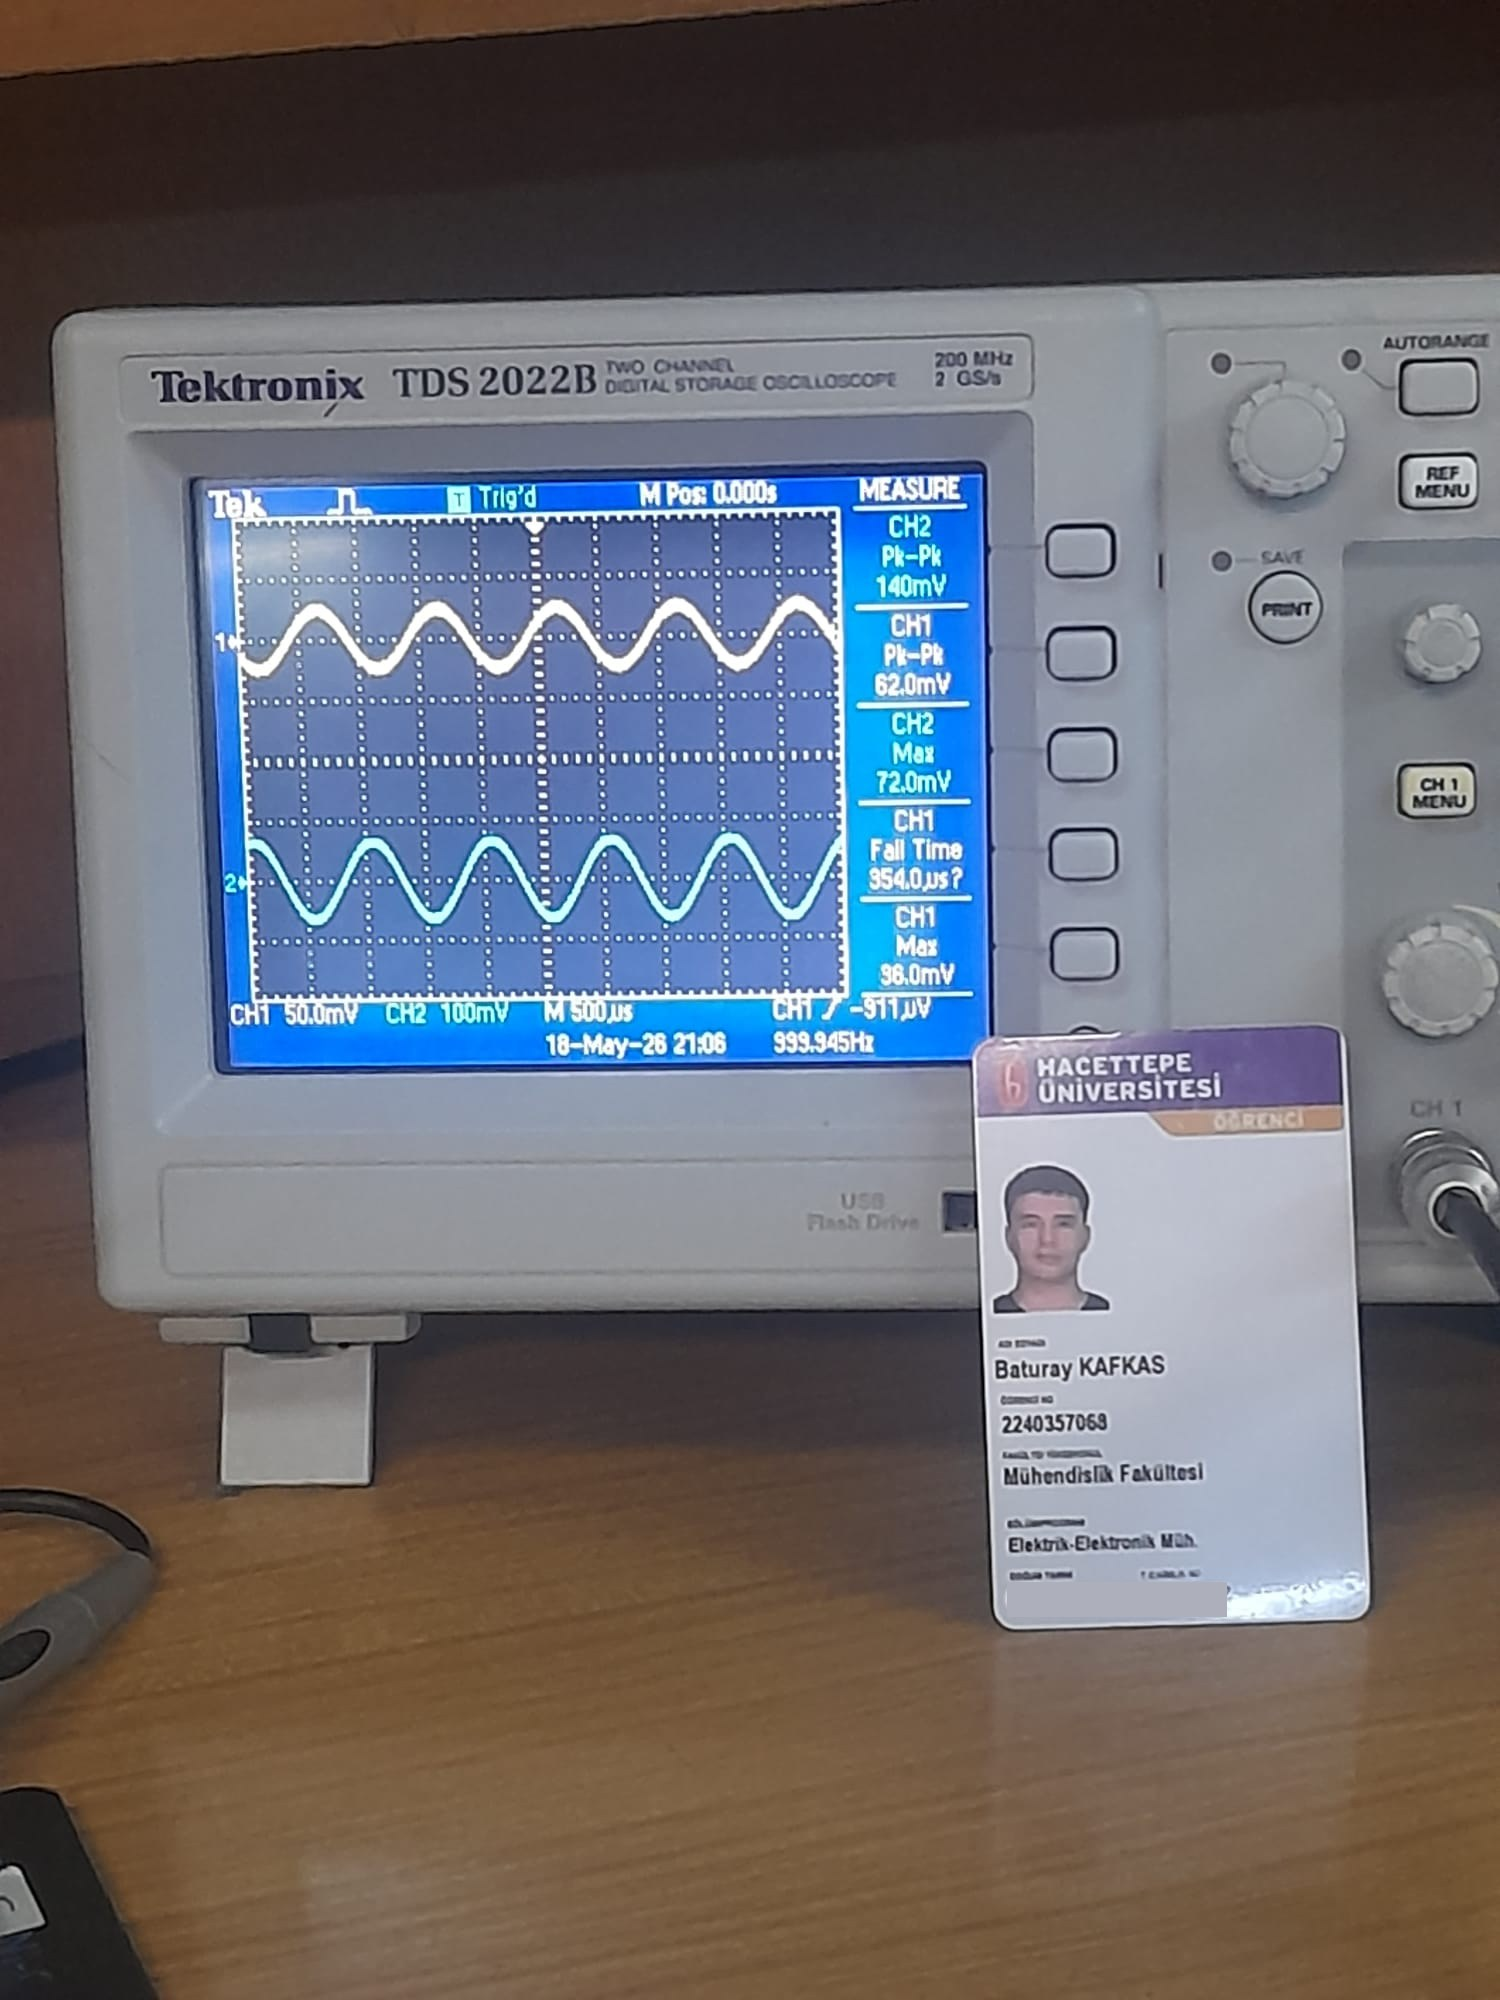
\includegraphics[width=\linewidth]{pertinax_circuit_meas2.jpg}
\captionof{figure}{Circuit Fabricated on a Pertinax Adjusted for Minimum Gain}
\label{fig:pertinax_circuit_meas2}
}
\vspace{1em}

\end{minipage}
\hfill
\begin{minipage}[t]{0.48\textwidth}
\vspace{0pt}
{
\centering
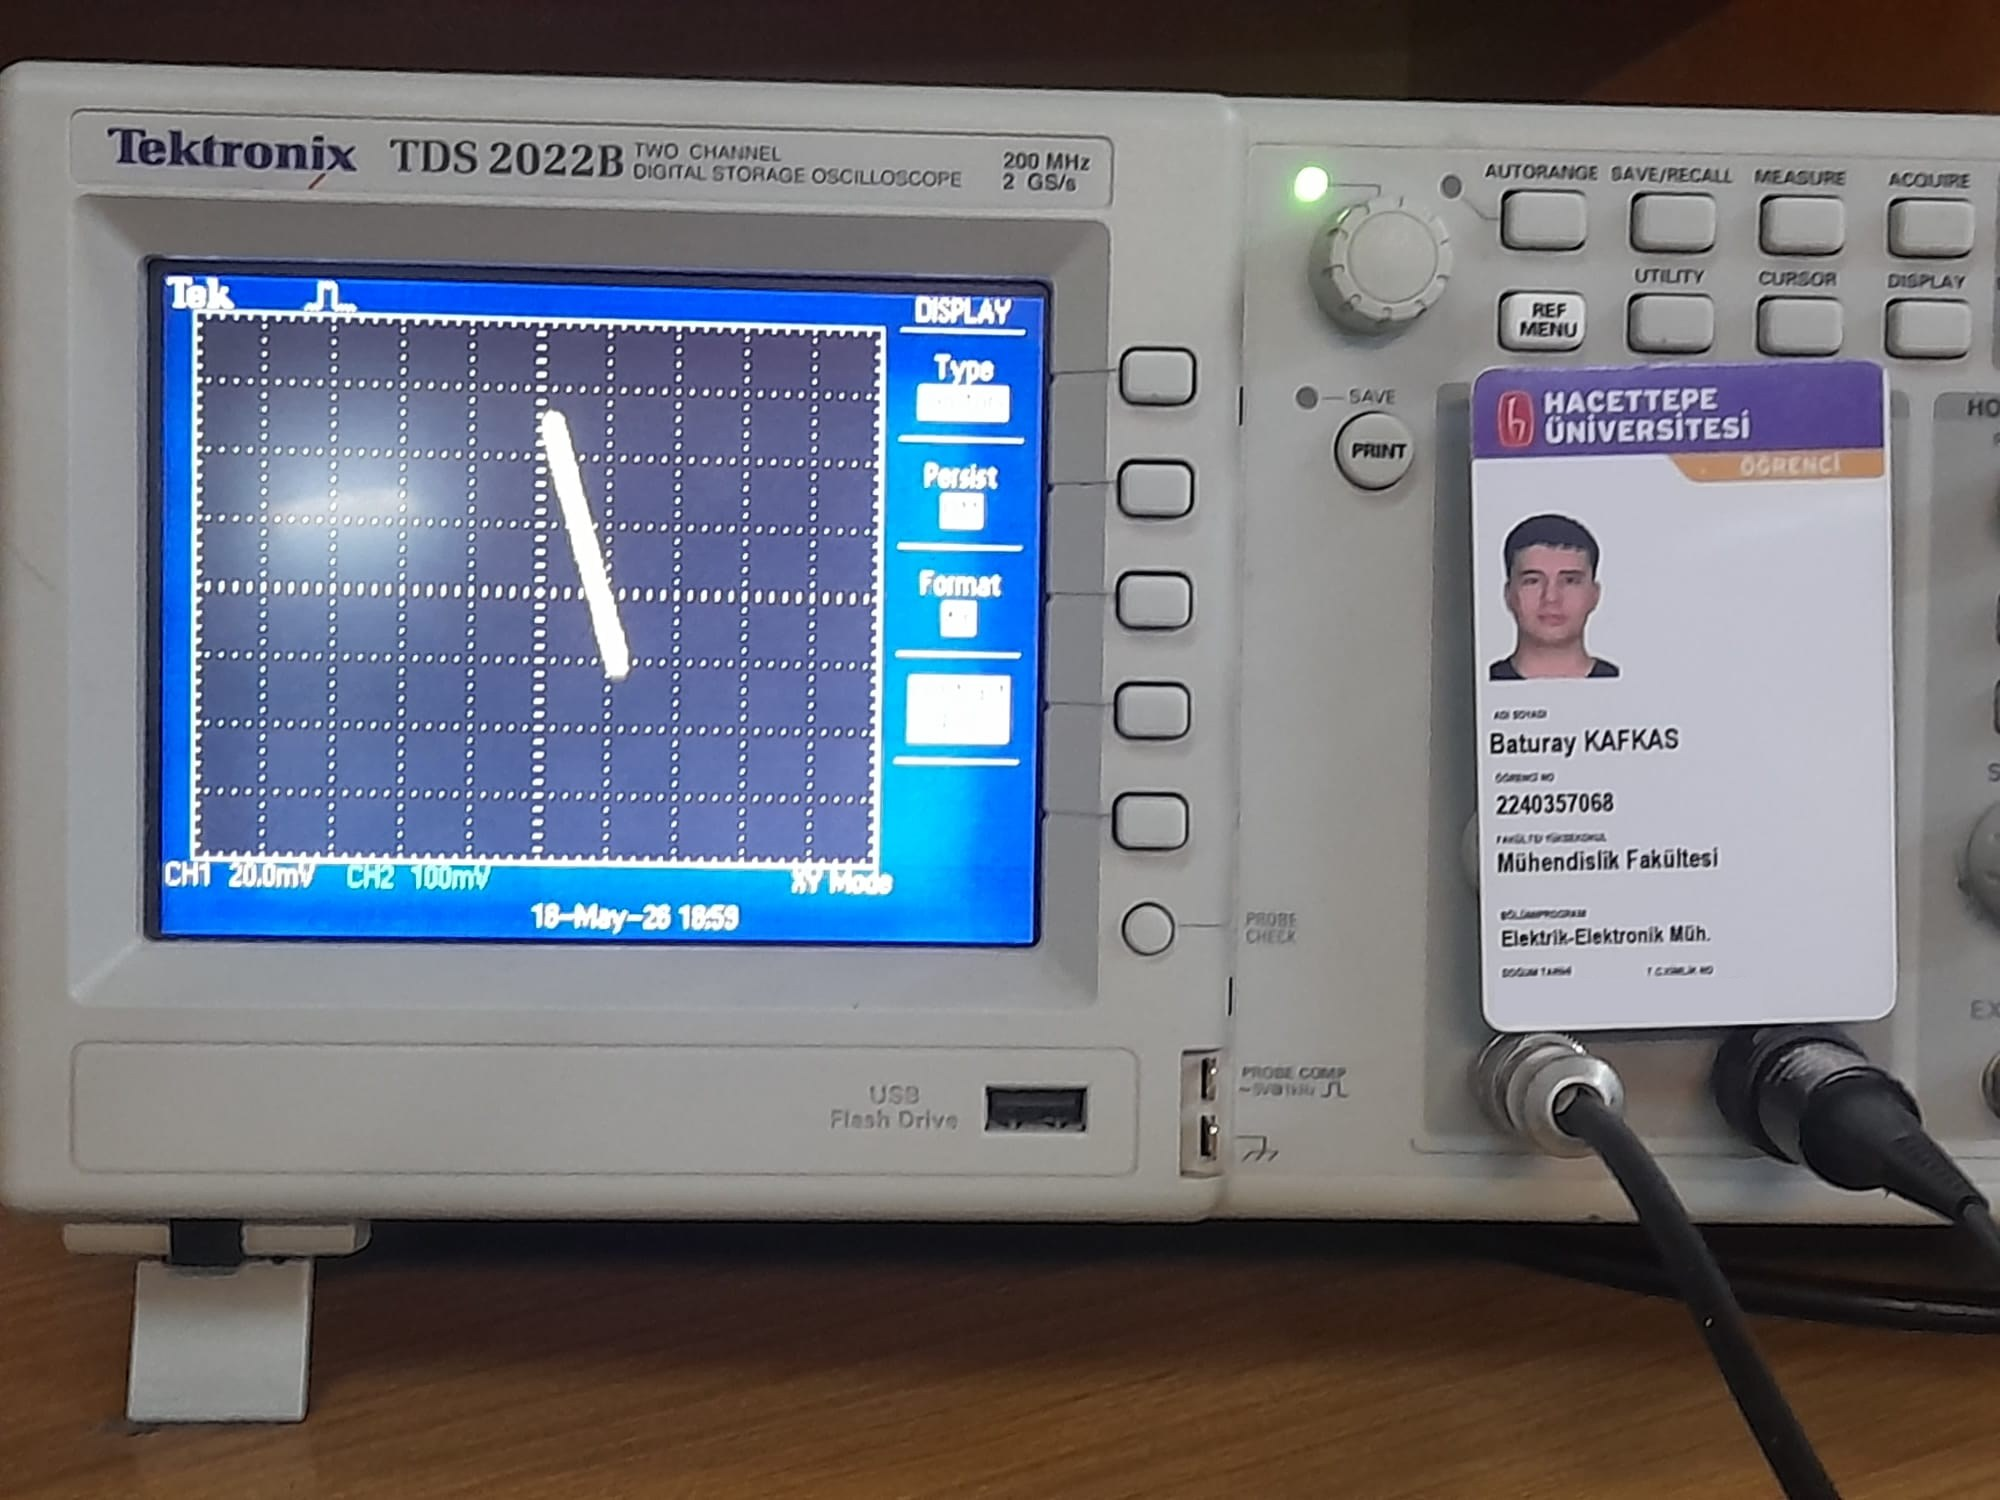
\includegraphics[width=\linewidth]{pertinax_circuit_meas3.jpg}
\captionof{figure}{Circuit Fabricated on a Pertinax Adjusted for Maximum Gain}
\label{fig:pertinax_circuit_meas3}
}
\vspace{1em}

We can obtain a minimum gain of
\[\left|A_{v,\text{ min}}\right|=140/62.0~\mathrm{V/V}\approx2.26~\mathrm{V/V}\]
and a maximum gain of roughly 
\[\left|A_{v,\text{ max}}\right|\approx350/20.0~\mathrm{V/V}=17.5~\mathrm{V/V}.\]
\end{minipage}

\autoref{fig:soldering} demonstrates the soldering process.

\begin{figure}[H]
    \centering
    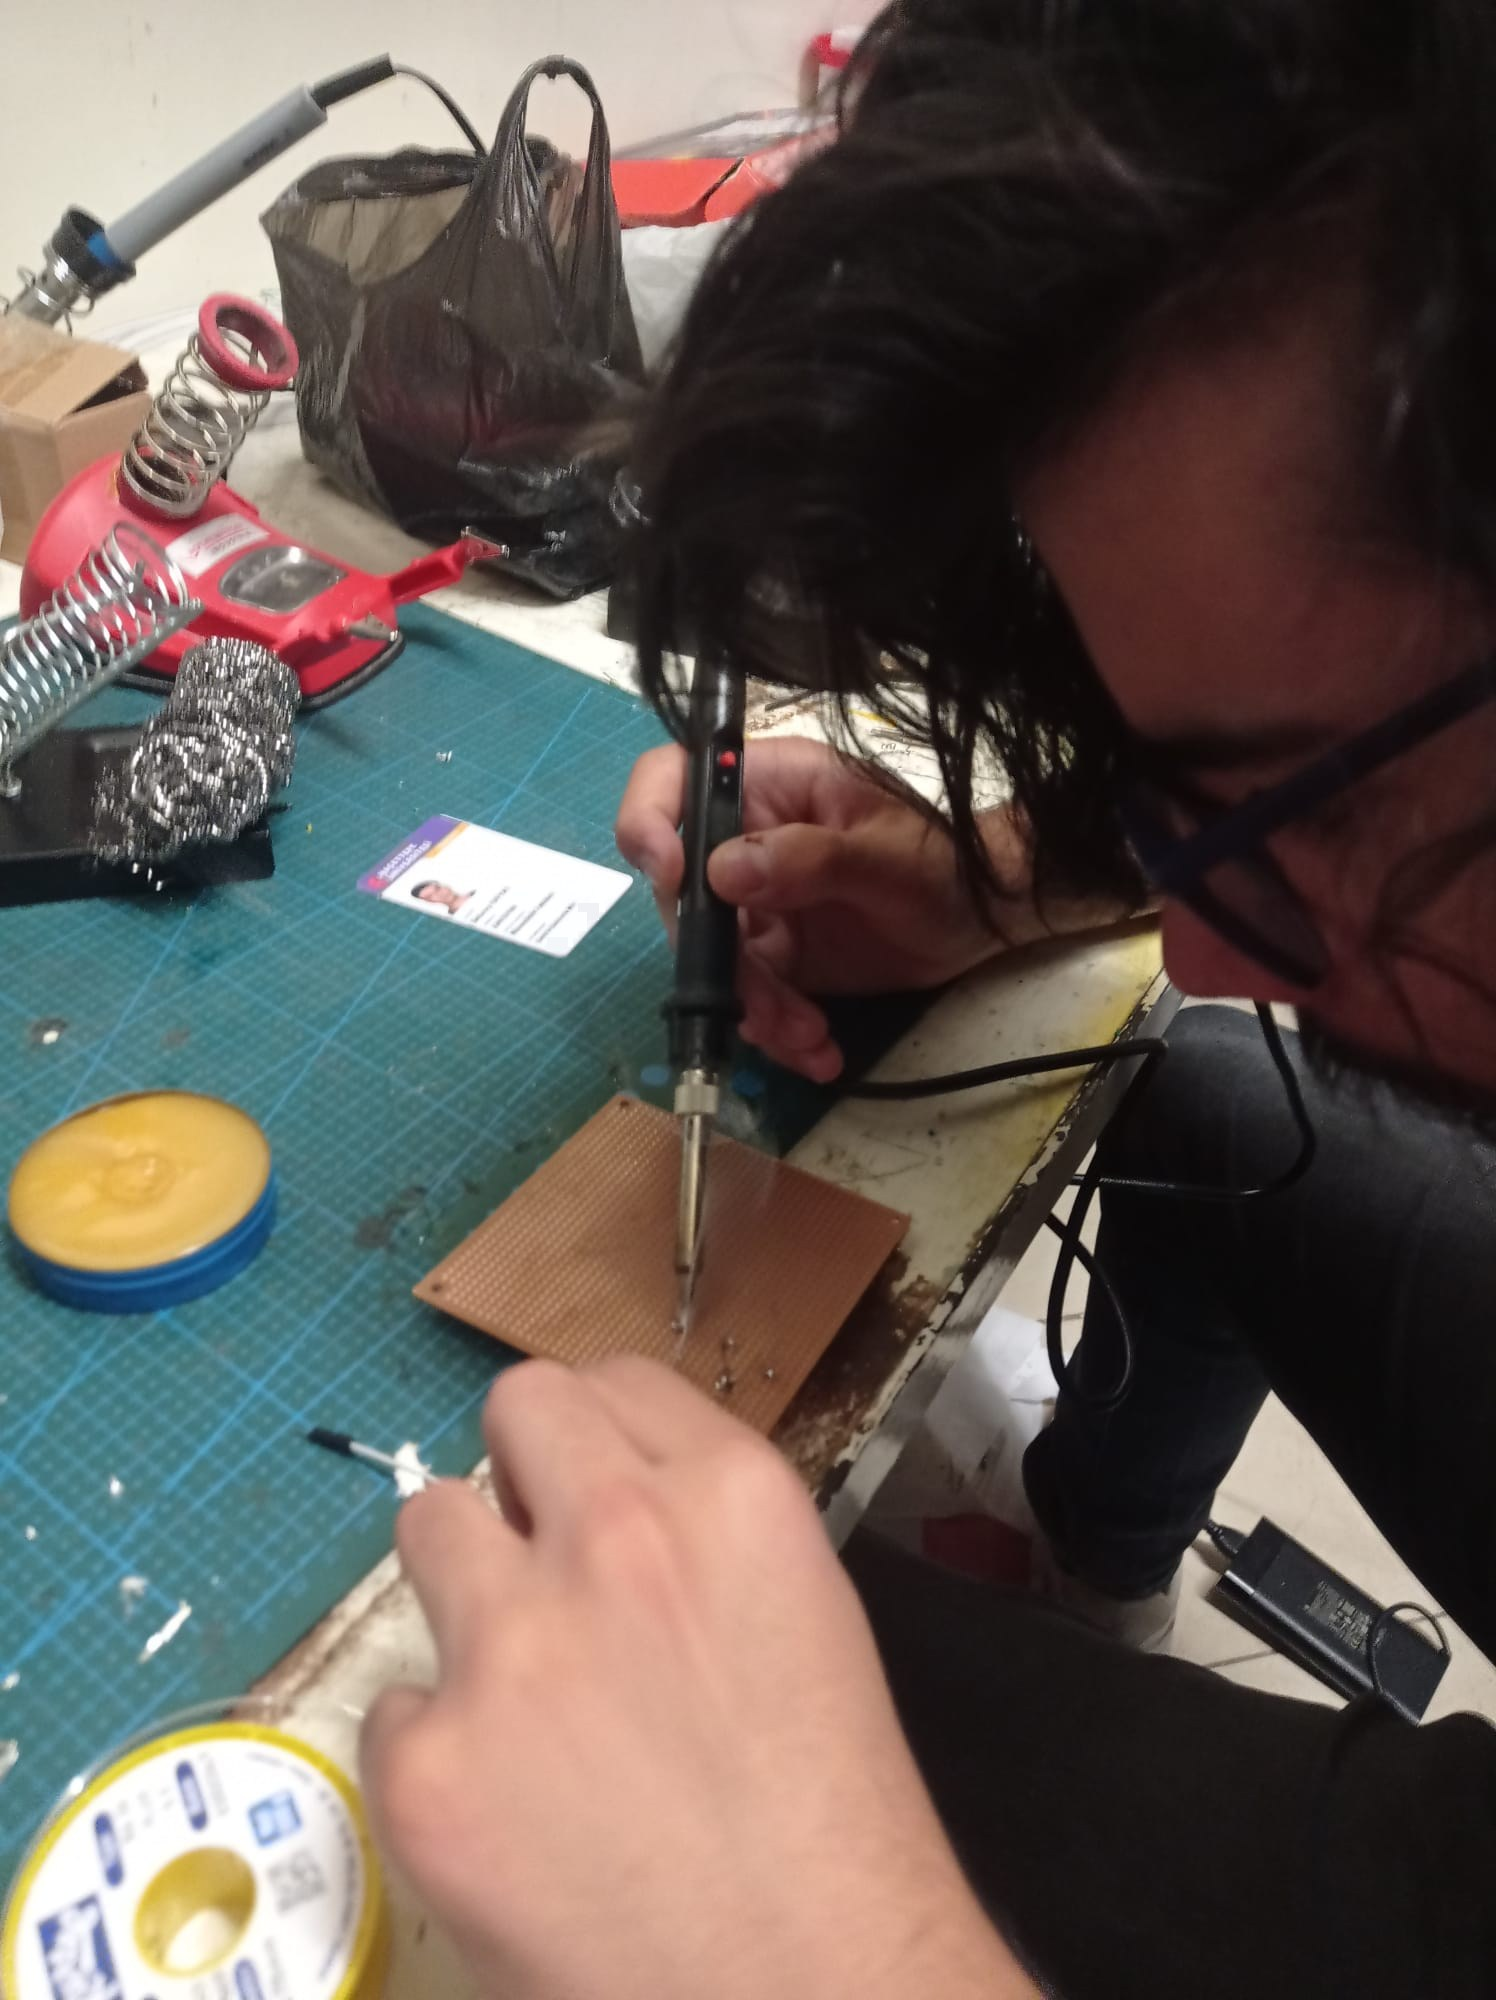
\includegraphics[width=0.48\linewidth]{soldering.jpg}

    \caption{Soldering Process}
    \label{fig:soldering}
\end{figure}

\section{Conclusion}

In this project, we managed to design, simulate and fabricate a multi-stage audio amplifier incorporating a BJT buffer stage, a passive band-pass equalizer stage, and a MOSFET gain stage without the use of operational amplifiers. The design combined semiconductor principles with practical circuit considerations to meet specific targets governed by the student ID parameters ($f_{low} = 680$~Hz, $f_{high} = 13200$~Hz, and a gain of $8$).

The selection of a 2N2222 BJT in an emitter-follower configuration effectively fulfilled the requirements of the buffer stage. The passive equalizer stage utilized linear and stable capacitive networks to form low- and high-pass filters, mitigating nonlinearities at the cost of minor signal attenuation ($\approx 9.8\%$). Finally, a 2N7000 NMOS transistor in a common-source configuration was employed, taking advantage of its exceptionally high gate isolation.

LTspice simulations confirmed the stable behavior of each individual block, yielding an equalizer bandpass close to theoretical values ($f_{lower}\approx706~\mathrm{Hz}$ and $f_{upper}\approx12.460~\mathrm{kHz}$). While the individual common-source configuration provided a peak localized gain of $A_v\approx-8.38~\mathrm{V/V}$, cascade loading interactions within the complete multistage layout resulted in a final simulated voltage gain of $A_v\approx-7.27~\mathrm{V/V}$ accompanied by the predicted $180^\circ$ phase inversion.

The most significant part of the assembly of the circuit on a Pertinax board was to apparently introduce a trimpot in series with the drain resistor to adjust the gain. The discrepancies between the analytical calculations, SPICE simulations, and final physical measurements can be attributed to factors such as internal component tolerances, parasitic contact resistances, and variations in transistor parameters. Eventually, the project successfully demonstrated the practical realization of discrete audio circuits.

\section{References}

\vspace{-3em}

\begin{thebibliography}{9}

\bibitem{1}
D. A. Neamen, “Basic BJT Amplifiers,” in *Design Application: Audio Amplifier*, 4th ed. New York, NY, USA: McGraw-Hill, 2010, pp. 445–449.

\bibitem{2}
“2N2222 PDF,” ALLDATASHEET.COM. [Online]. Available: \href{https://www.alldatasheet.com/datasheet-pdf/view/888490/SEMTECH_ELEC/2N2222.html}{\url{https://www.alldatasheet.com/datasheet-pdf/view/888490/SEMTECH_ELEC/2N2222.html}}. [Accessed: 16 May, 2026].

%onsemi, “2N2222A - NPN Bipolar Transistor,” datasheet, 2021. [Online]. Available: \href{https://www.onsemi.com/download/data-sheet/pdf/2n2222a-d.pdf}{\url{https://www.onsemi.com/download/data-sheet/pdf/2n2222a-d.pdf}}. [Accessed: May 2, 2026].

\bibitem{3}
onsemi, “NDS7002A - N-Channel Enhancement Mode Field Effect Transistor,” datasheet, 1998. [Online]. Available: \href{https://www.onsemi.com/download/data-sheet/pdf/nds7002a-d.pdf}{\url{https://www.onsemi.com/download/data-sheet/pdf/nds7002a-d.pdf}}. [Accessed: May 16, 2026].

\bibitem{4}
"Standard.mos," LTwiki. [Online]. Available: \href{https://ltwiki.org/index.php?title=Standard.mos}{\url{https://ltwiki.org/index.php?title=Standard.mos}}. [Accessed: May 16, 2026].
\end{thebibliography}

\appendix
\section{Handwritten Calculations and Schematics}
\label{subsec:appendix_a}

\begin{figure}[H]
    \centering
    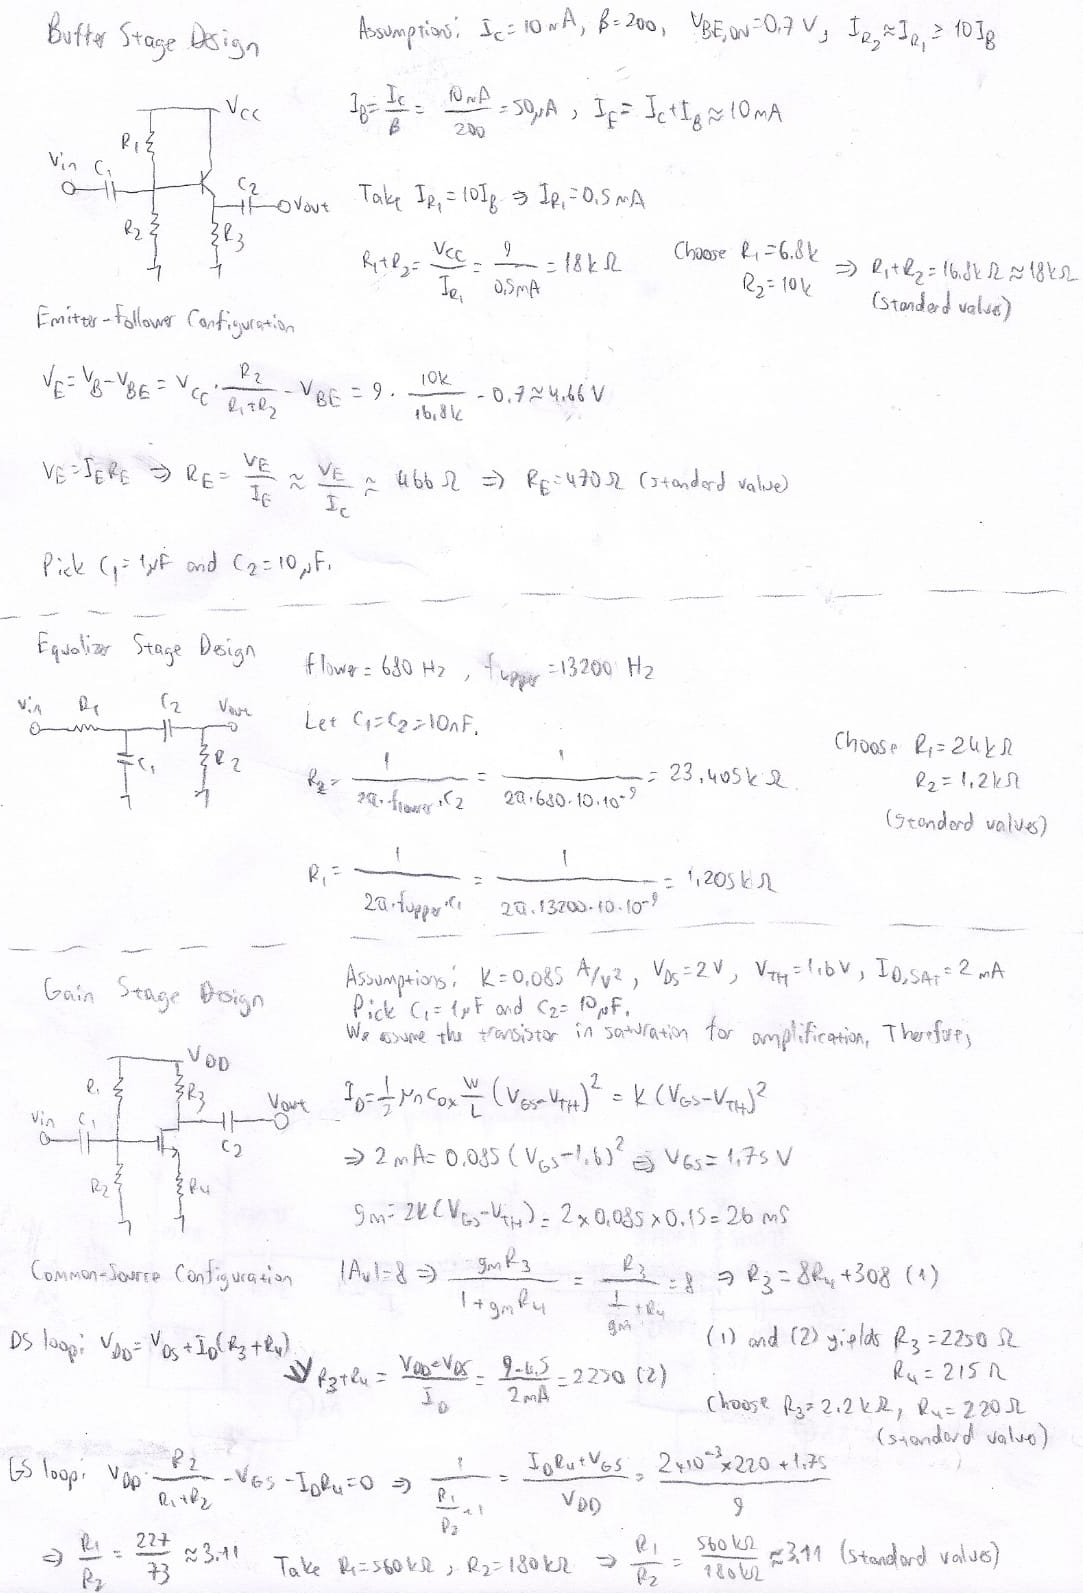
\includegraphics[width=0.97\linewidth]{calculations.png}

    \caption{Handwritten Analytical Calculations}
    \label{fig:fig_a1}
\end{figure}

\begin{figure}[H]
    \centering
    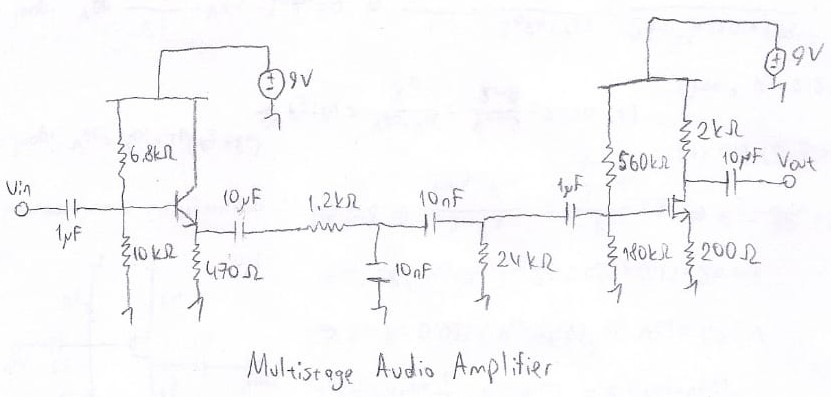
\includegraphics[width=1\linewidth]{multistage.jpeg}
    
    \caption{Handwritten Multistage Audio Amplifier}
    \label{fig:fig_a2}
\end{figure}

\section{Figures and Tables}

\label{subsec:appendix_b}

\begin{table}[H]
\centering
\caption{Timestamps for Fabrication and Testing Figures}
\label{tab:fabrication_timestamps}
\renewcommand{\arraystretch}{1.2}
\begin{tabularx}{\textwidth}{|l|X|c|}
\hline
\textbf{Figure} & \textbf{Description} & \textbf{Timestamp} \\ \hline
\ref{fig:buffer_stage_breadboard} & Buffer Stage on the Breadboard & 14/05/2026 18:23 \\ \hline
\ref{fig:buffer_stage_breadboard_meas} & Output Voltage of the Buffer Stage on the Breadboard & 14/05/2026 18:23 \\ \hline
\ref{fig:equalizer_stage_breadboard} & Equalizer Stage on the Breadboard & 14/05/2026 18:51 \\ \hline
\ref{fig:equalizer_stage_breadboard_meas1} & Equalizer Stage on the Breadboard Adjusted for Lower Cutoff Frequency & 14/05/2026 18:51 \\ \hline
\ref{fig:equalizer_stage_breadboard_meas2} & Equalizer Stage on the Breadboard Adjusted for Upper Cutoff Frequency & 14/05/2026 18:55 \\ \hline
\ref{fig:gain_stage_breadboard} & Gain Stage on the Breadboard & 14/05/2026 20:40 \\ \hline
\ref{fig:gain_stage_breadboard_meas} & Output Voltage of the Gain Stage on the Breadboard & 14/05/2026 20:40 \\ \hline
\ref{fig:multistage_breadboard_and_results} & Multistage Audio Amplifier on the Breadboard and its Testing & 14/05/2026 21:12 \\ \hline
\ref{fig:breadboard_debugging} & Breadboard Debugging & May 2026 \\ \hline
\ref{fig:breadboard_testing} & Breadboard Testing & May 2026 \\ \hline
\ref{fig:pertinax_circuit} & Circuit Fabricated on a Pertinax & 18/05/2026 14:50 \\ \hline
\ref{fig:pertinax_circuit_meas1} & Testing of the Circuit Fabricated on a Pertinax & 18/05/2026 11:16 \\ \hline
\ref{fig:pertinax_circuit_meas2} & Circuit Fabricated on a Pertinax Adjusted for Minimum Gain & 18/05/2026 14:43 \\ \hline
\ref{fig:pertinax_circuit_meas3} & Circuit Fabricated on a Pertinax Adjusted for Maximum Gain & 18/05/2026 12:36 \\ \hline
\ref{fig:soldering} & Soldering Process & May 2026 \\ \hline
\end{tabularx}
\end{table}

\newpage

\listoftables
\listoffigures

\end{document}